\graphicspath{{Ch5_VHqqbb/figures/}}

\chapter{All-Hadronic VH Resonance Search}

This thesis presents the ATLAS search for new resonances decaying to a vector boson $V = W,Z$ and a Standard Model (SM) Higgs boson $H$, in the fully hadronic $q\bar{q}^{(\prime)}b\bar{b}$ decay channels.
This search focuses on new resonance masses of $m_{VH} \geq 1.5$~TeV.
The $V$ and $H$ bosons that are produced in the decay of such heavy resonances are highly boosted and the resulting decay products of each boson are likely to be collimated and merged into a single large radius jet.
The dijet invariant mass spectrum of the two large radius jets is then used as discriminant variable, where the signature of the new heavy resonance decay yields a resonant structure on top of the smoothly falling background.
The dominant background ($\approx$ 90\%) corresponds to multijet QCD processes, with much smaller contributions from other non-resonant backgrounds: $t\bar{t}$ and $V$ + jets.
After reconstructing the $V$ and $H$ boson candidates as large radius jets, the tools of jet substructure and b-tagging are applied to heavily suppress the dominant background of multijet events.
Due to the challenges associated with modelling this background with Monte Carlo (MC) samples, a fully data-driven method is used to provide a background estimation method.

%TODO: define dijet mass very clearly

A simplified model \cite{Pappadopulo:2014qza} fulfilling only SM symmetry constraints is used to provide a model-independent Lagrangian for a heavy resonance search.
This framework incorporates Heavy Vector Triplets (HVT), a common SM extension with an isospin $SU(2)_{L}$ triplet formed of a neutral $Z'$ and two charged $W^{\prime \pm}$ bosons, from which two explicit models will be considered as benchmarks to evaluate the relative sensitivity of this analysis to $W^{\prime \pm}$ and $Z'$ signals: Models A and B \cite{Pappadopulo:2014qza}, where weakly and strongly coupling scenarios are described, respectively.
The couplings of the new vector bosons $W^{\prime \pm}$, $Z'$ to the $H$ and $V$ bosons are defined as a combination of parameters $g_{V}c_{H}$, while the couplings to fermions are defined as $(g^{2}/g_{V})c_{F}$, where $g_V$ represents the strength of the new vector boson interaction and $c_{H}$ ($c_{F}$) represents the coupling to the Higgs boson (fermions).
In Model A, the branching fractions to fermions and gauge bosons are comparable, whereas in Model B the fermionic couplings are suppressed.

A search for heavy vector resonances decaying to $VH$ in the fully hadronic final state was previously performed in ATLAS using $36.1\pm1.0\text{~fb}^{-1}$ of $pp$ collision data at 13 TeV taken during 2015 and 2016 \cite{Aaboud:2017ahz}.
The largest excess was observed in the $ZH$ channel at $m_{JJ}\sim3.0$~TeV with a local significance of 3.3~$\sigma$, with a  global significance of  2.2~$\sigma$.
Upper limits on the production cross-section times branching ratio to the $q\bar{q}^{(\prime)}b\bar{b}$ final state were set for resonance masses in the range between 1000 and 3800 GeV with values ranging between 107 to 3 fb and 97 to 2 fb (at 95\% CL) for $WH$ and $ZH$ resonances, respectively.
The corresponding excluded HVT Model B signal mass ranges are 1000-2500 GeV for $WH$ resonances, and 1000 - 2600 GeV for $ZH$ resonances.

Searches for heavy vector resonances decaying to $VH$ in the $V$ boson leptonic decay channels have been performed in ATLAS using $36.1\pm1.0\text{~fb}^{-1}$ of $pp$ collision data at 13 TeV \cite{EXOT-2016-10}.
For HVT Model A $W'$ ($Z'$) masses have been excluded up to 2.67 TeV (2.65 TeV), while for Model B, $W'$ ($Z'$) masses of up to 2.86 TeV (2.83 TeV) have been excluded.

The CMS collaboration has published a search for new heavy objects decaying to $VH$ in the fully hadronic mode using $19.7$~fb$^{-1}$ of 8 TeV data from Run 1 of the LHC.
Resonance masses up to 1.7 TeV were excluded in the combined $W'$ and $Z'$ search (1.1 TeV in \zpzh, 1.5 TeV in \wpwh), using the HVT Model B benchmark \cite{Khachatryan:2015bma}.
The search was also performed by CMS using $35.9$~fb$^{-1}$ of 13 TeV data from Run 2 of the LHC, excluding $W'$ ($Z'$) bosons with masses up to 3.15 TeV (2.26 TeV, except 1.19-1.21 TeV) in Model B \cite{Sirunyan:2017wto}.

% TODO: adapt this summary to thesis .tex structure
%This note is structured as follows: Section \ref{sec:samples} describes the data and simulated samples; Section \ref{sec:objects} and \ref{sec:selection} describe the object definitions and event selections and corresponding optimization studies; Section \ref{sec:background} describes the strategy for background estimation; Section \ref{sec:syst} describes the systematic uncertainties considered in this search; finally Sections \ref{sec:result} and \ref{sec:conclusion} present the results and conclusions of this search.

\section{Theoretical Motivation/Overview}
%TODO: describe HVT Model A/B distinction

\begin{figure}
	\centering
	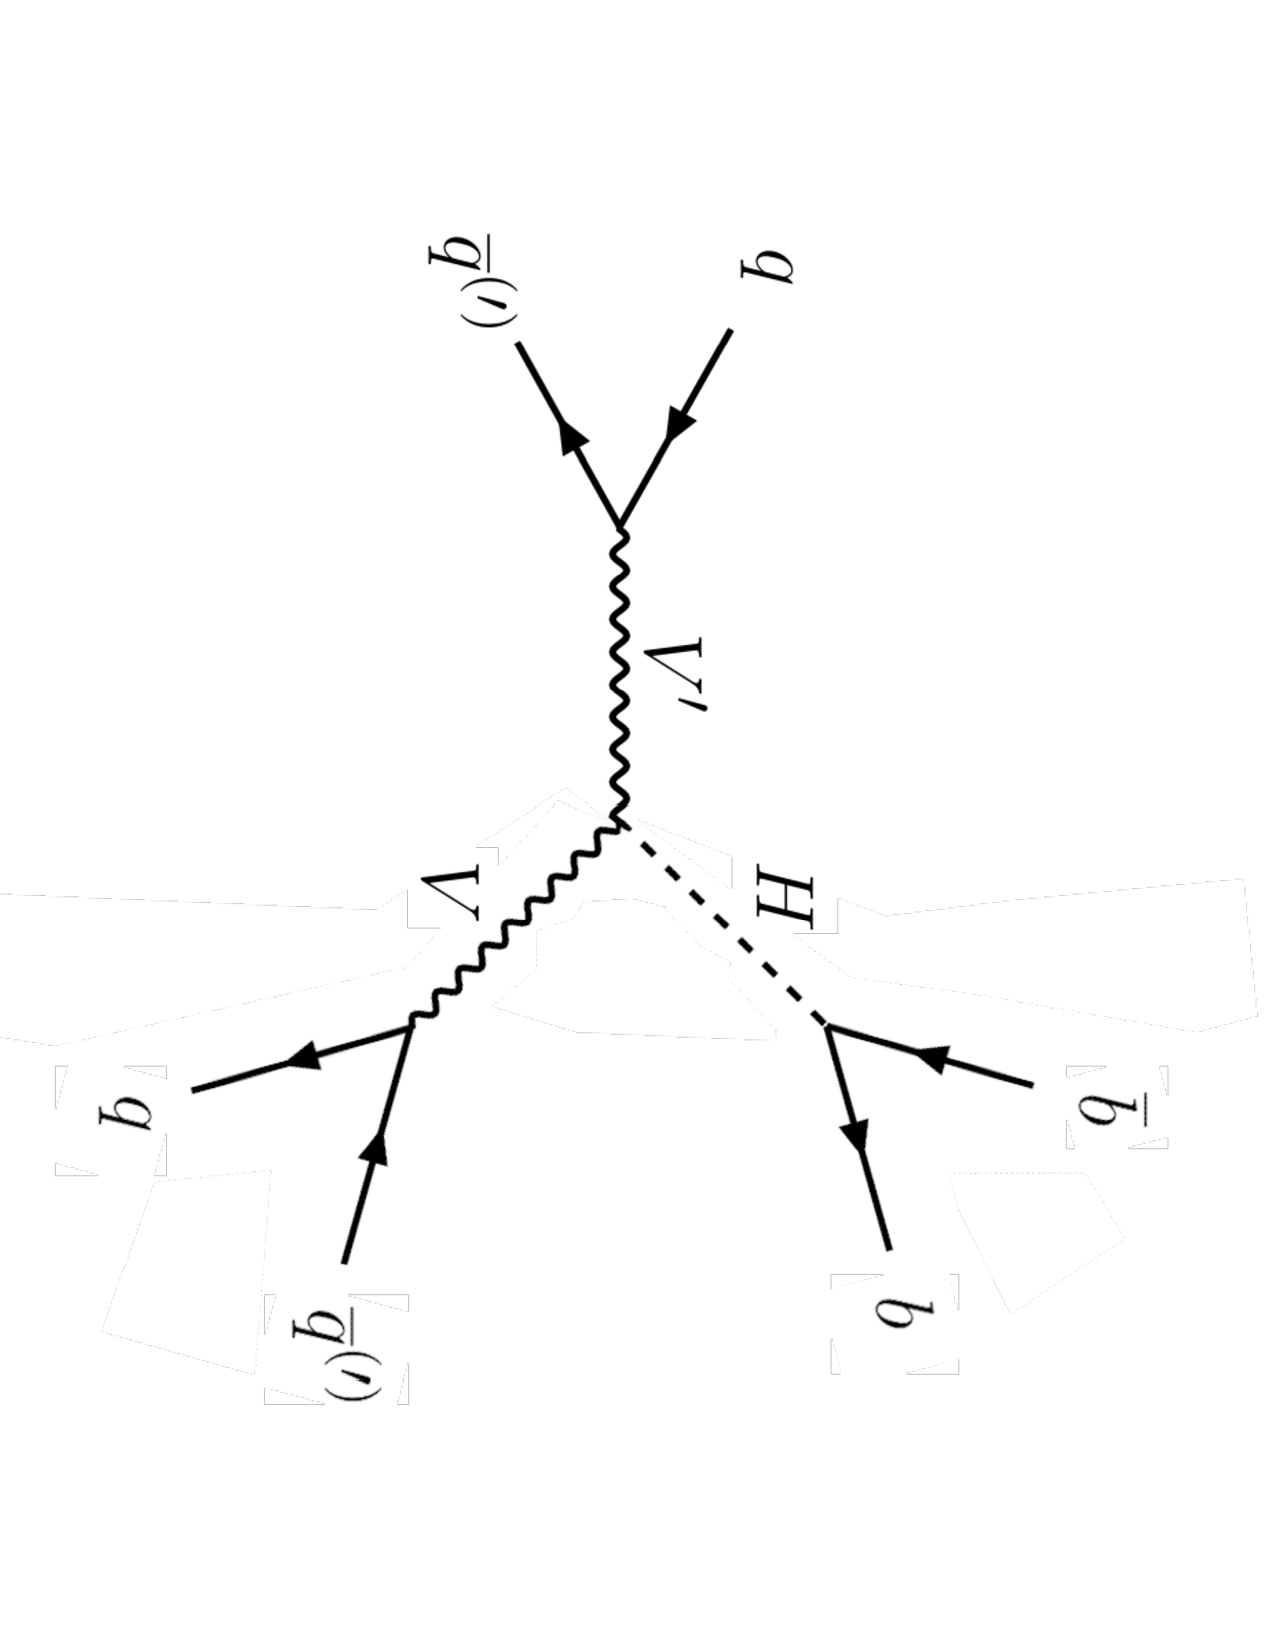
\includegraphics[width=0.75\textwidth,angle=90,origin=c]{feynman_diagram_VHqqbb}
	\caption{
	Feynman diagram illustrating the $pp \rightarrow V^\prime \rightarrow VH$ production/decay chain searched for in this analysis.
	}
	\label{fig:feynman_diagram_VHqqbb}
\end{figure}

\dots

\section{Analysis Strategy}
\dots

\section{Data and Simulated Samples}

Tables~\ref{tab:hvta_wh} and ~\ref{tab:hvta_zh} summarize the properties of the HVT Model A signal samples generated and used for this analysis, while Tables~\ref{tab:hvtb_wh} and ~\ref{tab:hvtb_zh} describe HVT Model B.

\begin{table}[!htb]
\begin{scriptsize}
\begin{center}
\begin{tabular}{|c|l|c|c|c|c|r|}
\hline
DSID & Process & Generator & $\sigma$ [fb] & $k$-factor & $\epsilon_{\text{filter}}$ & Events \\ \hline
302321 & \makecell{HVT $W^{\prime} \rightarrow WH \rightarrow qq^\prime(b\bar{b} + c\bar{c})$ \\ Model A, m = 1000 GeV} & \makecell{\MADGRAPH v2.2.2 + \PYTHIA v8.186 \\ + EvtGen v1.2.0} & 4.334e+02 & 1.0 & 1.0 & 110000 \\
\hline
302322 & \makecell{HVT $W^{\prime} \rightarrow WH \rightarrow qq^\prime(b\bar{b} + c\bar{c})$ \\ Model A, m = 1100 GeV} & \makecell{\MADGRAPH v2.2.2 + \PYTHIA v8.186 \\ + EvtGen v1.2.0} & 2.901e+02 & 1.0 & 1.0 & 110000 \\
\hline
302323 & \makecell{HVT $W^{\prime} \rightarrow WH \rightarrow qq^\prime(b\bar{b} + c\bar{c})$ \\ Model A, m = 1200 GeV} & \makecell{\MADGRAPH v2.2.2 + \PYTHIA v8.186 \\ + EvtGen v1.2.0} & 1.995e+02 & 1.0 & 1.0 & 110000 \\
\hline
302324 & \makecell{HVT $W^{\prime} \rightarrow WH \rightarrow qq^\prime(b\bar{b} + c\bar{c})$ \\ Model A, m = 1300 GeV} & \makecell{\MADGRAPH v2.2.2 + \PYTHIA v8.186 \\ + EvtGen v1.2.0} & 1.401e+02 & 1.0 & 1.0 & 95000 \\
\hline
302325 & \makecell{HVT $W^{\prime} \rightarrow WH \rightarrow qq^\prime(b\bar{b} + c\bar{c})$ \\ Model A, m = 1400 GeV} & \makecell{\MADGRAPH v2.2.2 + \PYTHIA v8.186 \\ + EvtGen v1.2.0} & 1.002e+02 & 1.0 & 1.0 & 125000 \\
\hline
302326 & \makecell{HVT $W^{\prime} \rightarrow WH \rightarrow qq^\prime(b\bar{b} + c\bar{c})$ \\ Model A, m = 1500 GeV} & \makecell{\MADGRAPH v2.2.2 + \PYTHIA v8.186 \\ + EvtGen v1.2.0} & 7.283e+01 & 1.0 & 1.0 & 80000 \\
\hline
302327 & \makecell{HVT $W^{\prime} \rightarrow WH \rightarrow qq^\prime(b\bar{b} + c\bar{c})$ \\ Model A, m = 1600 GeV} & \makecell{\MADGRAPH v2.2.3 + \PYTHIA v8.186 \\ + EvtGen v1.2.0} & 5.367e+01 & 1.0 & 1.0 & 110000 \\
\hline
302328 & \makecell{HVT $W^{\prime} \rightarrow WH \rightarrow qq^\prime(b\bar{b} + c\bar{c})$ \\ Model A, m = 1700 GeV} & \makecell{\MADGRAPH v2.2.2 + \PYTHIA v8.186 \\ + EvtGen v1.2.0} & 3.999e+01 & 1.0 & 1.0 & 110000 \\
\hline
302329 & \makecell{HVT $W^{\prime} \rightarrow WH \rightarrow qq^\prime(b\bar{b} + c\bar{c})$ \\ Model A, m = 1800 GeV} & \makecell{\MADGRAPH v2.2.3 + \PYTHIA v8.186 \\ + EvtGen v1.2.0} & 3.012e+01 & 1.0 & 1.0 & 110000 \\
\hline
302330 & \makecell{HVT $W^{\prime} \rightarrow WH \rightarrow qq^\prime(b\bar{b} + c\bar{c})$ \\ Model A, m = 1900 GeV} & \makecell{\MADGRAPH v2.2.2 + \PYTHIA v8.186 \\ + EvtGen v1.2.0} & 2.289e+01 & 1.0 & 1.0 & 70000 \\
\hline
302331 & \makecell{HVT $W^{\prime} \rightarrow WH \rightarrow qq^\prime(b\bar{b} + c\bar{c})$ \\ Model A, m = 2000 GeV} & \makecell{\MADGRAPH v2.2.2 + \PYTHIA v8.186 \\ + EvtGen v1.2.0} & 1.753e+01 & 1.0 & 1.0 & 105000 \\
\hline
302332 & \makecell{HVT $W^{\prime} \rightarrow WH \rightarrow qq^\prime(b\bar{b} + c\bar{c})$ \\ Model A, m = 2200 GeV} & \makecell{\MADGRAPH v2.2.2 + \PYTHIA v8.186 \\ + EvtGen v1.2.0} & 1.049e+01 & 1.0 & 1.0 & 110000 \\
\hline
302333 & \makecell{HVT $W^{\prime} \rightarrow WH \rightarrow qq^\prime(b\bar{b} + c\bar{c})$ \\ Model A, m = 2400 GeV} & \makecell{\MADGRAPH v2.2.2 + \PYTHIA v8.186 \\ + EvtGen v1.2.0} & 6.427e+00 & 1.0 & 1.0 & 110000 \\
\hline
302334 & \makecell{HVT $W^{\prime} \rightarrow WH \rightarrow qq^\prime(b\bar{b} + c\bar{c})$ \\ Model A, m = 2600 GeV} & \makecell{\MADGRAPH v2.2.2 + \PYTHIA v8.186 \\ + EvtGen v1.2.0} & 4.008e+00 & 1.0 & 1.0 & 110000 \\
\hline
302335 & \makecell{HVT $W^{\prime} \rightarrow WH \rightarrow qq^\prime(b\bar{b} + c\bar{c})$ \\ Model A, m = 2800 GeV} & \makecell{\MADGRAPH v2.2.2 + \PYTHIA v8.186 \\ + EvtGen v1.2.0} & 2.537e+00 & 1.0 & 1.0 & 110000 \\
\hline
302336 & \makecell{HVT $W^{\prime} \rightarrow WH \rightarrow qq^\prime(b\bar{b} + c\bar{c})$ \\ Model A, m = 3000 GeV} & \makecell{\MADGRAPH v2.2.2 + \PYTHIA v8.186 \\ + EvtGen v1.2.0} & 1.624e+00 & 1.0 & 1.0 & 50000 \\
\hline
302337 & \makecell{HVT $W^{\prime} \rightarrow WH \rightarrow qq^\prime(b\bar{b} + c\bar{c})$ \\ Model A, m = 3500 GeV} & \makecell{\MADGRAPH v2.2.2 + \PYTHIA v8.186 \\ + EvtGen v1.2.0} & 5.534e-01 & 1.0 & 1.0 & 65000 \\
\hline
302338 & \makecell{HVT $W^{\prime} \rightarrow WH \rightarrow qq^\prime(b\bar{b} + c\bar{c})$ \\ Model A, m = 4000 GeV} & \makecell{\MADGRAPH v2.2.2 + \PYTHIA v8.186 \\ + EvtGen v1.2.0} & 1.953e-01 & 1.0 & 1.0 & 100000 \\
\hline
302339 & \makecell{HVT $W^{\prime} \rightarrow WH \rightarrow qq^\prime(b\bar{b} + c\bar{c})$ \\ Model A, m = 4500 GeV} & \makecell{\MADGRAPH v2.2.2 + \PYTHIA v8.186 \\ + EvtGen v1.2.0} & 7.015e-02 & 1.0 & 1.0 & 80000 \\
\hline
302340 & \makecell{HVT $W^{\prime} \rightarrow WH \rightarrow qq^\prime(b\bar{b} + c\bar{c})$ \\ Model A, m = 5000 GeV} & \makecell{\MADGRAPH v2.2.2 + \PYTHIA v8.186 \\ + EvtGen v1.2.0} & 2.543e-02 & 1.0 & 1.0 & 85000 \\
\hline
\end{tabular}
\caption{
    HVT Model A ($g_V=1$) WH samples used in the analysis. The dataset ID, MC generator, production cross-sections,
    $k$-factor, filter efficiency and total number of generated events are shown.
}
\label{tab:hvta_wh}
\end{center}
\end{scriptsize}
\end{table}

\begin{table}[!htb]
\begin{scriptsize}
\begin{center}
\begin{tabular}{|c|l|c|c|c|c|r|}
\hline
DSID & Process & Generator & $\sigma$ [fb] & $k$-factor & $\epsilon_{\text{filter}}$ & Events \\ \hline
302371 & \makecell{HVT $Z^{\prime} \rightarrow ZH \rightarrow q\bar{q}(b\bar{b} + c\bar{c})$ \\ Model A, m = 1000 GeV} & \makecell{\MADGRAPH v2.2.2 + \PYTHIA v8.186 \\ + EvtGen v1.2.0} & 2.179e+02 & 1.0 & 1.0 & 50000 \\
\hline
302372 & \makecell{HVT $Z^{\prime} \rightarrow ZH \rightarrow q\bar{q}(b\bar{b} + c\bar{c})$ \\ Model A, m = 1100 GeV} & \makecell{\MADGRAPH v2.2.3 + \PYTHIA v8.186 \\ + EvtGen v1.2.0} & 1.446e+02 & 1.0 & 1.0 & 110000 \\
\hline
302373 & \makecell{HVT $Z^{\prime} \rightarrow ZH \rightarrow q\bar{q}(b\bar{b} + c\bar{c})$ \\ Model A, m = 1200 GeV} & \makecell{\MADGRAPH v2.2.2 + \PYTHIA v8.186 \\ + EvtGen v1.2.0} & 9.855e+01 & 1.0 & 1.0 & 80000 \\
\hline
302374 & \makecell{HVT $Z^{\prime} \rightarrow ZH \rightarrow q\bar{q}(b\bar{b} + c\bar{c})$ \\ Model A, m = 1300 GeV} & \makecell{\MADGRAPH v2.2.2 + \PYTHIA v8.186 \\ + EvtGen v1.2.0} & 6.871e+01 & 1.0 & 1.0 & 70000 \\
\hline
302375 & \makecell{HVT $Z^{\prime} \rightarrow ZH \rightarrow q\bar{q}(b\bar{b} + c\bar{c})$ \\ Model A, m = 1400 GeV} & \makecell{\MADGRAPH v2.2.2 + \PYTHIA v8.186 \\ + EvtGen v1.2.0} & 4.881e+01 & 1.0 & 1.0 & 95000 \\
\hline
302376 & \makecell{HVT $Z^{\prime} \rightarrow ZH \rightarrow q\bar{q}(b\bar{b} + c\bar{c})$ \\ Model A, m = 1500 GeV} & \makecell{\MADGRAPH v2.2.2 + \PYTHIA v8.186 \\ + EvtGen v1.2.0} & 3.525e+01 & 1.0 & 1.0 & 100000 \\
\hline
302377 & \makecell{HVT $Z^{\prime} \rightarrow ZH \rightarrow q\bar{q}(b\bar{b} + c\bar{c})$ \\ Model A, m = 1600 GeV} & \makecell{\MADGRAPH v2.2.2 + \PYTHIA v8.186 \\ + EvtGen v1.2.0} & 2.581e+01 & 1.0 & 1.0 & 55000 \\
\hline
302378 & \makecell{HVT $Z^{\prime} \rightarrow ZH \rightarrow q\bar{q}(b\bar{b} + c\bar{c})$ \\ Model A, m = 1700 GeV} & \makecell{\MADGRAPH v2.2.3 + \PYTHIA v8.186 \\ + EvtGen v1.2.0} & 1.913e+01 & 1.0 & 1.0 & 110000 \\
\hline
302379 & \makecell{HVT $Z^{\prime} \rightarrow ZH \rightarrow q\bar{q}(b\bar{b} + c\bar{c})$ \\ Model A, m = 1800 GeV} & \makecell{\MADGRAPH v2.2.2 + \PYTHIA v8.186 \\ + EvtGen v1.2.0} & 1.434e+01 & 1.0 & 1.0 & 104000 \\
\hline
302380 & \makecell{HVT $Z^{\prime} \rightarrow ZH \rightarrow q\bar{q}(b\bar{b} + c\bar{c})$ \\ Model A, m = 1900 GeV} & \makecell{\MADGRAPH v2.2.2 + \PYTHIA v8.186 \\ + EvtGen v1.2.0} & 1.084e+01 & 1.0 & 1.0 & 95000 \\
\hline
302381 & \makecell{HVT $Z^{\prime} \rightarrow ZH \rightarrow q\bar{q}(b\bar{b} + c\bar{c})$ \\ Model A, m = 2000 GeV} & \makecell{\MADGRAPH v2.2.2 + \PYTHIA v8.186 \\ + EvtGen v1.2.0} & 8.271e+00 & 1.0 & 1.0 & 110000 \\
\hline
302382 & \makecell{HVT $Z^{\prime} \rightarrow ZH \rightarrow q\bar{q}(b\bar{b} + c\bar{c})$ \\ Model A, m = 2200 GeV} & \makecell{\MADGRAPH v2.2.2 + \PYTHIA v8.186 \\ + EvtGen v1.2.0} & 4.916e+00 & 1.0 & 1.0 & 85000 \\
\hline
302383 & \makecell{HVT $Z^{\prime} \rightarrow ZH \rightarrow q\bar{q}(b\bar{b} + c\bar{c})$ \\ Model A, m = 2400 GeV} & \makecell{\MADGRAPH v2.2.3 + \PYTHIA v8.186 \\ + EvtGen v1.2.0} & 2.994e+00 & 1.0 & 1.0 & 110000 \\
\hline
302384 & \makecell{HVT $Z^{\prime} \rightarrow ZH \rightarrow q\bar{q}(b\bar{b} + c\bar{c})$ \\ Model A, m = 2600 GeV} & \makecell{\MADGRAPH v2.2.2 + \PYTHIA v8.186 \\ + EvtGen v1.2.0} & 1.859e+00 & 1.0 & 1.0 & 105000 \\
\hline
302385 & \makecell{HVT $Z^{\prime} \rightarrow ZH \rightarrow q\bar{q}(b\bar{b} + c\bar{c})$ \\ Model A, m = 2800 GeV} & \makecell{\MADGRAPH v2.2.2 + \PYTHIA v8.186 \\ + EvtGen v1.2.0} & 1.173e+00 & 1.0 & 1.0 & 70000 \\
\hline
302386 & \makecell{HVT $Z^{\prime} \rightarrow ZH \rightarrow q\bar{q}(b\bar{b} + c\bar{c})$ \\ Model A, m = 3000 GeV} & \makecell{\MADGRAPH v2.2.2 + \PYTHIA v8.186 \\ + EvtGen v1.2.0} & 7.497e-01 & 1.0 & 1.0 & 90000 \\
\hline
302387 & \makecell{HVT $Z^{\prime} \rightarrow ZH \rightarrow q\bar{q}(b\bar{b} + c\bar{c})$ \\ Model A, m = 3500 GeV} & \makecell{\MADGRAPH v2.2.2 + \PYTHIA v8.186 \\ + EvtGen v1.2.0} & 2.554e-01 & 1.0 & 1.0 & 110000 \\
\hline
302388 & \makecell{HVT $Z^{\prime} \rightarrow ZH \rightarrow q\bar{q}(b\bar{b} + c\bar{c})$ \\ Model A, m = 4000 GeV} & \makecell{\MADGRAPH v2.2.2 + \PYTHIA v8.186 \\ + EvtGen v1.2.0} & 9.049e-02 & 1.0 & 1.0 & 75000 \\
\hline
302389 & \makecell{HVT $Z^{\prime} \rightarrow ZH \rightarrow q\bar{q}(b\bar{b} + c\bar{c})$ \\ Model A, m = 4500 GeV} & \makecell{\MADGRAPH v2.2.2 + \PYTHIA v8.186 \\ + EvtGen v1.2.0} & 3.274e-02 & 1.0 & 1.0 & 100000 \\
\hline
302390 & \makecell{HVT $Z^{\prime} \rightarrow ZH \rightarrow q\bar{q}(b\bar{b} + c\bar{c})$ \\ Model A, m = 5000 GeV} & \makecell{\MADGRAPH v2.2.2 + \PYTHIA v8.186 \\ + EvtGen v1.2.0} & 1.198e-02 & 1.0 & 1.0 & 110000 \\
\hline
\end{tabular}
\caption{
    HVT Model A ($g_V=1$) ZH samples used in the analysis. The dataset ID, MC generator, production cross-sections,
    $k$-factor, filter efficiency and total number of generated events are shown.
}
\label{tab:hvta_zh}
\end{center}
\end{scriptsize}
\end{table}

\begin{table}[!htb]
\begin{scriptsize}
\begin{center}
\begin{tabular}{|c|l|c|c|c|c|r|}
\hline
DSID & Process & Generator & $\sigma$ [fb] & $k$-factor & $\epsilon_{\text{filter}}$ & Events \\ \hline
302321 & \makecell{HVT $W^{\prime} \rightarrow WH \rightarrow qq^\prime(b\bar{b} + c\bar{c})$ \\ Model B, m = 1000 GeV} & \makecell{\MADGRAPH v2.2.2 + \PYTHIA v8.186 \\ + EvtGen v1.2.0} & 5.016e+02 & 1.0 & 1.0 & 110000 \\
\hline
302322 & \makecell{HVT $W^{\prime} \rightarrow WH \rightarrow qq^\prime(b\bar{b} + c\bar{c})$ \\ Model B, m = 1100 GeV} & \makecell{\MADGRAPH v2.2.2 + \PYTHIA v8.186 \\ + EvtGen v1.2.0} & 3.634e+02 & 1.0 & 1.0 & 110000 \\
\hline
302323 & \makecell{HVT $W^{\prime} \rightarrow WH \rightarrow qq^\prime(b\bar{b} + c\bar{c})$ \\ Model B, m = 1200 GeV} & \makecell{\MADGRAPH v2.2.2 + \PYTHIA v8.186 \\ + EvtGen v1.2.0} & 2.646e+02 & 1.0 & 1.0 & 110000 \\
\hline
302324 & \makecell{HVT $W^{\prime} \rightarrow WH \rightarrow qq^\prime(b\bar{b} + c\bar{c})$ \\ Model B, m = 1300 GeV} & \makecell{\MADGRAPH v2.2.2 + \PYTHIA v8.186 \\ + EvtGen v1.2.0} & 1.943e+02 & 1.0 & 1.0 & 95000 \\
\hline
302325 & \makecell{HVT $W^{\prime} \rightarrow WH \rightarrow qq^\prime(b\bar{b} + c\bar{c})$ \\ Model B, m = 1400 GeV} & \makecell{\MADGRAPH v2.2.2 + \PYTHIA v8.186 \\ + EvtGen v1.2.0} & 1.440e+02 & 1.0 & 1.0 & 125000 \\
\hline
302326 & \makecell{HVT $W^{\prime} \rightarrow WH \rightarrow qq^\prime(b\bar{b} + c\bar{c})$ \\ Model B, m = 1500 GeV} & \makecell{\MADGRAPH v2.2.2 + \PYTHIA v8.186 \\ + EvtGen v1.2.0} & 1.077e+02 & 1.0 & 1.0 & 80000 \\
\hline
302327 & \makecell{HVT $W^{\prime} \rightarrow WH \rightarrow qq^\prime(b\bar{b} + c\bar{c})$ \\ Model B, m = 1600 GeV} & \makecell{\MADGRAPH v2.2.3 + \PYTHIA v8.186 \\ + EvtGen v1.2.0} & 8.128e+01 & 1.0 & 1.0 & 110000 \\
\hline
302328 & \makecell{HVT $W^{\prime} \rightarrow WH \rightarrow qq^\prime(b\bar{b} + c\bar{c})$ \\ Model B, m = 1700 GeV} & \makecell{\MADGRAPH v2.2.2 + \PYTHIA v8.186 \\ + EvtGen v1.2.0} & 6.181e+01 & 1.0 & 1.0 & 110000 \\
\hline
302329 & \makecell{HVT $W^{\prime} \rightarrow WH \rightarrow qq^\prime(b\bar{b} + c\bar{c})$ \\ Model B, m = 1800 GeV} & \makecell{\MADGRAPH v2.2.3 + \PYTHIA v8.186 \\ + EvtGen v1.2.0} & 4.733e+01 & 1.0 & 1.0 & 110000 \\
\hline
302330 & \makecell{HVT $W^{\prime} \rightarrow WH \rightarrow qq^\prime(b\bar{b} + c\bar{c})$ \\ Model B, m = 1900 GeV} & \makecell{\MADGRAPH v2.2.2 + \PYTHIA v8.186 \\ + EvtGen v1.2.0} & 3.648e+01 & 1.0 & 1.0 & 70000 \\
\hline
302331 & \makecell{HVT $W^{\prime} \rightarrow WH \rightarrow qq^\prime(b\bar{b} + c\bar{c})$ \\ Model B, m = 2000 GeV} & \makecell{\MADGRAPH v2.2.2 + \PYTHIA v8.186 \\ + EvtGen v1.2.0} & 2.827e+01 & 1.0 & 1.0 & 105000 \\
\hline
302332 & \makecell{HVT $W^{\prime} \rightarrow WH \rightarrow qq^\prime(b\bar{b} + c\bar{c})$ \\ Model B, m = 2200 GeV} & \makecell{\MADGRAPH v2.2.2 + \PYTHIA v8.186 \\ + EvtGen v1.2.0} & 1.723e+01 & 1.0 & 1.0 & 110000 \\
\hline
302333 & \makecell{HVT $W^{\prime} \rightarrow WH \rightarrow qq^\prime(b\bar{b} + c\bar{c})$ \\ Model B, m = 2400 GeV} & \makecell{\MADGRAPH v2.2.2 + \PYTHIA v8.186 \\ + EvtGen v1.2.0} & 1.067e+01 & 1.0 & 1.0 & 110000 \\
\hline
% 308541 & \makecell{HVT $W^{\prime} \rightarrow WH \rightarrow qq^\prime(b\bar{b} + c\bar{c})$ \\ Model B, m = 2500 GeV} & \makecell{\MADGRAPH v2.3.3 + \PYTHIA v8.212 \\ + EvtGen v1.6.0} & 8.443e+00 & 1.0 & 1.0 & 100000 \\
% \hline
302334 & \makecell{HVT $W^{\prime} \rightarrow WH \rightarrow qq^\prime(b\bar{b} + c\bar{c})$ \\ Model B, m = 2600 GeV} & \makecell{\MADGRAPH v2.2.2 + \PYTHIA v8.186 \\ + EvtGen v1.2.0} & 6.689e+00 & 1.0 & 1.0 & 110000 \\
\hline
% 308542 & \makecell{HVT $W^{\prime} \rightarrow WH \rightarrow qq^\prime(b\bar{b} + c\bar{c})$ \\ Model B, m = 2700 GeV} & \makecell{\MADGRAPH v2.3.3 + \PYTHIA v8.212 \\ + EvtGen v1.6.0} & 5.317e+00 & 1.0 & 1.0 & 110000 \\
% \hline
302335 & \makecell{HVT $W^{\prime} \rightarrow WH \rightarrow qq^\prime(b\bar{b} + c\bar{c})$ \\ Model B, m = 2800 GeV} & \makecell{\MADGRAPH v2.2.2 + \PYTHIA v8.186 \\ + EvtGen v1.2.0} & 4.234e+00 & 1.0 & 1.0 & 110000 \\
\hline
%308543 & \makecell{HVT $W^{\prime} \rightarrow WH \rightarrow qq^\prime(b\bar{b} + c\bar{c})$ \\ Model B, m = 2900 GeV} & \makecell{\MADGRAPH v2.3.3 + \PYTHIA v8.212 \\ + EvtGen v1.6.0} & 3.377e+00 & 1.0 & 1.0 & 110000 \\
%\hline
302336 & \makecell{HVT $W^{\prime} \rightarrow WH \rightarrow qq^\prime(b\bar{b} + c\bar{c})$ \\ Model B, m = 3000 GeV} & \makecell{\MADGRAPH v2.2.2 + \PYTHIA v8.186 \\ + EvtGen v1.2.0} & 2.698e+00 & 1.0 & 1.0 & 50000 \\
\hline
% 308544 & \makecell{HVT $W^{\prime} \rightarrow WH \rightarrow qq^\prime(b\bar{b} + c\bar{c})$ \\ Model B, m = 3100 GeV} & \makecell{\MADGRAPH v2.3.3 + \PYTHIA v8.212 \\ + EvtGen v1.6.0} & 2.159e+00 & 1.0 & 1.0 & 110000 \\
% \hline
% 306776 & \makecell{HVT $W^{\prime} \rightarrow WH \rightarrow qq^\prime(b\bar{b} + c\bar{c})$ \\ Model B, m = 3200 GeV} & \makecell{\MADGRAPH v2.3.3 + \PYTHIA v8.212 \\ + EvtGen v1.2.0} & 1.729e+00 & 1.0 & 1.0 & 109000 \\
% \hline
%308545 & \makecell{HVT $W^{\prime} \rightarrow WH \rightarrow qq^\prime(b\bar{b} + c\bar{c})$ \\ Model B, m = 3300 GeV} & \makecell{\MADGRAPH v2.3.3 + \PYTHIA v8.212 \\ + EvtGen v1.6.0} & 1.386e+00 & 1.0 & 1.0 & 110000 \\
%\hline
%306777 & \makecell{HVT $W^{\prime} \rightarrow WH \rightarrow qq^\prime(b\bar{b} + c\bar{c})$ \\ Model B, m = 3400 GeV} & \makecell{\MADGRAPH v2.3.3 + \PYTHIA v8.212 \\ + EvtGen v1.2.0} & 1.111e+00 & 1.0 & 1.0 & 110000 \\
%\hline
302337 & \makecell{HVT $W^{\prime} \rightarrow WH \rightarrow qq^\prime(b\bar{b} + c\bar{c})$ \\ Model B, m = 3500 GeV} & \makecell{\MADGRAPH v2.2.2 + \PYTHIA v8.186 \\ + EvtGen v1.2.0} & 8.918e-01 & 1.0 & 1.0 & 65000 \\
\hline
%306778 & \makecell{HVT $W^{\prime} \rightarrow WH \rightarrow qq^\prime(b\bar{b} + c\bar{c})$ \\ Model B, m = 3600 GeV} & \makecell{\MADGRAPH v2.3.3 + \PYTHIA v8.212 \\ + EvtGen v1.2.0} & 7.157e-01 & 1.0 & 1.0 & 110000 \\
%\hline
%306779 & \makecell{HVT $W^{\prime} \rightarrow WH \rightarrow qq^\prime(b\bar{b} + c\bar{c})$ \\ Model B, m = 3800 GeV} & \makecell{\MADGRAPH v2.3.3 + \PYTHIA v8.212 \\ + EvtGen v1.2.0} & 4.611e-01 & 1.0 & 1.0 & 110000 \\
%\hline
302338 & \makecell{HVT $W^{\prime} \rightarrow WH \rightarrow qq^\prime(b\bar{b} + c\bar{c})$ \\ Model B, m = 4000 GeV} & \makecell{\MADGRAPH v2.2.2 + \PYTHIA v8.186 \\ + EvtGen v1.2.0} & 2.969e-01 & 1.0 & 1.0 & 100000 \\
\hline
302339 & \makecell{HVT $W^{\prime} \rightarrow WH \rightarrow qq^\prime(b\bar{b} + c\bar{c})$ \\ Model B, m = 4500 GeV} & \makecell{\MADGRAPH v2.2.2 + \PYTHIA v8.186 \\ + EvtGen v1.2.0} & 9.789e-02 & 1.0 & 1.0 & 80000 \\
\hline
302340 & \makecell{HVT $W^{\prime} \rightarrow WH \rightarrow qq^\prime(b\bar{b} + c\bar{c})$ \\ Model B, m = 5000 GeV} & \makecell{\MADGRAPH v2.2.2 + \PYTHIA v8.186 \\ + EvtGen v1.2.0} & 3.149e-02 & 1.0 & 1.0 & 85000 \\
\hline
\end{tabular}
\caption{
    HVT Model B ($g_V=3$) WH samples used in the analysis. The dataset ID, MC generator, production cross-sections,
    $k$-factor, filter efficiency and total number of generated events are shown.
}
\label{tab:hvtb_wh}
\end{center}
\end{scriptsize}
\end{table}

\begin{table}[!htb]
\begin{scriptsize}
\begin{center}
\begin{tabular}{|c|l|c|c|c|c|r|}
\hline
DSID & Process & Generator & $\sigma$ [fb] & $k$-factor & $\epsilon_{\text{filter}}$ & Events \\ \hline
302371 & \makecell{HVT $Z^{\prime} \rightarrow ZH \rightarrow q\bar{q}(b\bar{b} + c\bar{c})$ \\ Model B, m = 1000 GeV} & \makecell{\MADGRAPH v2.2.2 + \PYTHIA v8.186 \\ + EvtGen v1.2.0} & 2.641e+02 & 1.0 & 1.0 & 50000 \\
\hline
302372 & \makecell{HVT $Z^{\prime} \rightarrow ZH \rightarrow q\bar{q}(b\bar{b} + c\bar{c})$ \\ Model B, m = 1100 GeV} & \makecell{\MADGRAPH v2.2.3 + \PYTHIA v8.186 \\ + EvtGen v1.2.0} & 1.888e+02 & 1.0 & 1.0 & 110000 \\
\hline
302373 & \makecell{HVT $Z^{\prime} \rightarrow ZH \rightarrow q\bar{q}(b\bar{b} + c\bar{c})$ \\ Model B, m = 1200 GeV} & \makecell{\MADGRAPH v2.2.2 + \PYTHIA v8.186 \\ + EvtGen v1.2.0} & 1.358e+02 & 1.0 & 1.0 & 80000 \\
\hline
302374 & \makecell{HVT $Z^{\prime} \rightarrow ZH \rightarrow q\bar{q}(b\bar{b} + c\bar{c})$ \\ Model B, m = 1300 GeV} & \makecell{\MADGRAPH v2.2.2 + \PYTHIA v8.186 \\ + EvtGen v1.2.0} & 9.864e+01 & 1.0 & 1.0 & 70000 \\
\hline
302375 & \makecell{HVT $Z^{\prime} \rightarrow ZH \rightarrow q\bar{q}(b\bar{b} + c\bar{c})$ \\ Model B, m = 1400 GeV} & \makecell{\MADGRAPH v2.2.2 + \PYTHIA v8.186 \\ + EvtGen v1.2.0} & 7.236e+01 & 1.0 & 1.0 & 95000 \\
\hline
302376 & \makecell{HVT $Z^{\prime} \rightarrow ZH \rightarrow q\bar{q}(b\bar{b} + c\bar{c})$ \\ Model B, m = 1500 GeV} & \makecell{\MADGRAPH v2.2.2 + \PYTHIA v8.186 \\ + EvtGen v1.2.0} & 5.359e+01 & 1.0 & 1.0 & 100000 \\
\hline
302377 & \makecell{HVT $Z^{\prime} \rightarrow ZH \rightarrow q\bar{q}(b\bar{b} + c\bar{c})$ \\ Model B, m = 1600 GeV} & \makecell{\MADGRAPH v2.2.2 + \PYTHIA v8.186 \\ + EvtGen v1.2.0} & 4.006e+01 & 1.0 & 1.0 & 55000 \\
\hline
302378 & \makecell{HVT $Z^{\prime} \rightarrow ZH \rightarrow q\bar{q}(b\bar{b} + c\bar{c})$ \\ Model B, m = 1700 GeV} & \makecell{\MADGRAPH v2.2.3 + \PYTHIA v8.186 \\ + EvtGen v1.2.0} & 3.020e+01 & 1.0 & 1.0 & 110000 \\
\hline
302379 & \makecell{HVT $Z^{\prime} \rightarrow ZH \rightarrow q\bar{q}(b\bar{b} + c\bar{c})$ \\ Model B, m = 1800 GeV} & \makecell{\MADGRAPH v2.2.2 + \PYTHIA v8.186 \\ + EvtGen v1.2.0} & 2.292e+01 & 1.0 & 1.0 & 104000 \\
\hline
302380 & \makecell{HVT $Z^{\prime} \rightarrow ZH \rightarrow q\bar{q}(b\bar{b} + c\bar{c})$ \\ Model B, m = 1900 GeV} & \makecell{\MADGRAPH v2.2.2 + \PYTHIA v8.186 \\ + EvtGen v1.2.0} & 1.752e+01 & 1.0 & 1.0 & 95000 \\
\hline
302381 & \makecell{HVT $Z^{\prime} \rightarrow ZH \rightarrow q\bar{q}(b\bar{b} + c\bar{c})$ \\ Model B, m = 2000 GeV} & \makecell{\MADGRAPH v2.2.2 + \PYTHIA v8.186 \\ + EvtGen v1.2.0} & 1.348e+01 & 1.0 & 1.0 & 110000 \\
\hline
302382 & \makecell{HVT $Z^{\prime} \rightarrow ZH \rightarrow q\bar{q}(b\bar{b} + c\bar{c})$ \\ Model B, m = 2200 GeV} & \makecell{\MADGRAPH v2.2.2 + \PYTHIA v8.186 \\ + EvtGen v1.2.0} & 8.102e+00 & 1.0 & 1.0 & 85000 \\
\hline
302383 & \makecell{HVT $Z^{\prime} \rightarrow ZH \rightarrow q\bar{q}(b\bar{b} + c\bar{c})$ \\ Model B, m = 2400 GeV} & \makecell{\MADGRAPH v2.2.3 + \PYTHIA v8.186 \\ + EvtGen v1.2.0} & 4.958e+00 & 1.0 & 1.0 & 110000 \\
\hline
%308546 & \makecell{HVT $Z^{\prime} \rightarrow ZH \rightarrow q\bar{q}(b\bar{b} + c\bar{c})$ \\ Model B, m = 2500 GeV} & \makecell{\MADGRAPH v2.3.3 + \PYTHIA v8.212 \\ + EvtGen v1.6.0} & 3.900e+00 & 1.0 & 1.0 & 100000 \\
%\hline
302384 & \makecell{HVT $Z^{\prime} \rightarrow ZH \rightarrow q\bar{q}(b\bar{b} + c\bar{c})$ \\ Model B, m = 2600 GeV} & \makecell{\MADGRAPH v2.2.2 + \PYTHIA v8.186 \\ + EvtGen v1.2.0} & 3.078e+00 & 1.0 & 1.0 & 105000 \\
\hline
%308547 & \makecell{HVT $Z^{\prime} \rightarrow ZH \rightarrow q\bar{q}(b\bar{b} + c\bar{c})$ \\ Model B, m = 2700 GeV} & \makecell{\MADGRAPH v2.3.3 + \PYTHIA v8.212 \\ + EvtGen v1.6.0} & 2.436e+00 & 1.0 & 1.0 & 110000 \\
%\hline
302385 & \makecell{HVT $Z^{\prime} \rightarrow ZH \rightarrow q\bar{q}(b\bar{b} + c\bar{c})$ \\ Model B, m = 2800 GeV} & \makecell{\MADGRAPH v2.2.2 + \PYTHIA v8.186 \\ + EvtGen v1.2.0} & 1.934e+00 & 1.0 & 1.0 & 70000 \\
\hline
%308548 & \makecell{HVT $Z^{\prime} \rightarrow ZH \rightarrow q\bar{q}(b\bar{b} + c\bar{c})$ \\ Model B, m = 2900 GeV} & \makecell{\MADGRAPH v2.3.3 + \PYTHIA v8.212 \\ + EvtGen v1.6.0} & 1.540e+00 & 1.0 & 1.0 & 109000 \\
%\hline
302386 & \makecell{HVT $Z^{\prime} \rightarrow ZH \rightarrow q\bar{q}(b\bar{b} + c\bar{c})$ \\ Model B, m = 3000 GeV} & \makecell{\MADGRAPH v2.2.2 + \PYTHIA v8.186 \\ + EvtGen v1.2.0} & 1.226e+00 & 1.0 & 1.0 & 90000 \\
\hline
%308549 & \makecell{HVT $Z^{\prime} \rightarrow ZH \rightarrow q\bar{q}(b\bar{b} + c\bar{c})$ \\ Model B, m = 3100 GeV} & \makecell{\MADGRAPH v2.3.3 + \PYTHIA v8.212 \\ + EvtGen v1.6.0} & 9.792e-01 & 1.0 & 1.0 & 110000 \\
%\hline
%306780 & \makecell{HVT $Z^{\prime} \rightarrow ZH \rightarrow q\bar{q}(b\bar{b} + c\bar{c})$ \\ Model B, m = 3200 GeV} & \makecell{\MADGRAPH v2.3.3 + \PYTHIA v8.212 \\ + EvtGen v1.2.0} & 7.835e-01 & 1.0 & 1.0 & 110000 \\
%\hline
%308550 & \makecell{HVT $Z^{\prime} \rightarrow ZH \rightarrow q\bar{q}(b\bar{b} + c\bar{c})$ \\ Model B, m = 3300 GeV} & \makecell{\MADGRAPH v2.3.3 + \PYTHIA v8.212 \\ + EvtGen v1.6.0} & 6.278e-01 & 1.0 & 1.0 & 105000 \\
%\hline
%306781 & \makecell{HVT $Z^{\prime} \rightarrow ZH \rightarrow q\bar{q}(b\bar{b} + c\bar{c})$ \\ Model B, m = 3400 GeV} & \makecell{\MADGRAPH v2.3.3 + \PYTHIA v8.212 \\ + EvtGen v1.2.0} & 5.037e-01 & 1.0 & 1.0 & 110000 \\
%\hline
302387 & \makecell{HVT $Z^{\prime} \rightarrow ZH \rightarrow q\bar{q}(b\bar{b} + c\bar{c})$ \\ Model B, m = 3500 GeV} & \makecell{\MADGRAPH v2.2.2 + \PYTHIA v8.186 \\ + EvtGen v1.2.0} & 4.046e-01 & 1.0 & 1.0 & 110000 \\
\hline
%306782 & \makecell{HVT $Z^{\prime} \rightarrow ZH \rightarrow q\bar{q}(b\bar{b} + c\bar{c})$ \\ Model B, m = 3600 GeV} & \makecell{\MADGRAPH v2.3.3 + \PYTHIA v8.212 \\ + EvtGen v1.2.0} & 3.253e-01 & 1.0 & 1.0 & 109000 \\
%\hline
%306783 & \makecell{HVT $Z^{\prime} \rightarrow ZH \rightarrow q\bar{q}(b\bar{b} + c\bar{c})$ \\ Model B, m = 3800 GeV} & \makecell{\MADGRAPH v2.3.3 + \PYTHIA v8.212 \\ + EvtGen v1.2.0} & 2.108e-01 & 1.0 & 1.0 & 110000 \\
%\hline
302388 & \makecell{HVT $Z^{\prime} \rightarrow ZH \rightarrow q\bar{q}(b\bar{b} + c\bar{c})$ \\ Model B, m = 4000 GeV} & \makecell{\MADGRAPH v2.2.2 + \PYTHIA v8.186 \\ + EvtGen v1.2.0} & 1.369e-01 & 1.0 & 1.0 & 75000 \\
\hline
302389 & \makecell{HVT $Z^{\prime} \rightarrow ZH \rightarrow q\bar{q}(b\bar{b} + c\bar{c})$ \\ Model B, m = 4500 GeV} & \makecell{\MADGRAPH v2.2.2 + \PYTHIA v8.186 \\ + EvtGen v1.2.0} & 4.673e-02 & 1.0 & 1.0 & 100000 \\
\hline
302390 & \makecell{HVT $Z^{\prime} \rightarrow ZH \rightarrow q\bar{q}(b\bar{b} + c\bar{c})$ \\ Model B, m = 5000 GeV} & \makecell{\MADGRAPH v2.2.2 + \PYTHIA v8.186 \\ + EvtGen v1.2.0} & 1.589e-02 & 1.0 & 1.0 & 110000 \\
\hline
\end{tabular}
\caption{
    HVT Model B ($g_V=3$) ZH samples used in the analysis. The dataset ID, MC generator, production cross-sections,
    $k$-factor, filter efficiency and total number of generated events are shown.
}
\label{tab:hvtb_zh}
\end{center}
\end{scriptsize}
\end{table}

\subsection{Data}

\begin{figure}[htbp!]
\begin{center}
    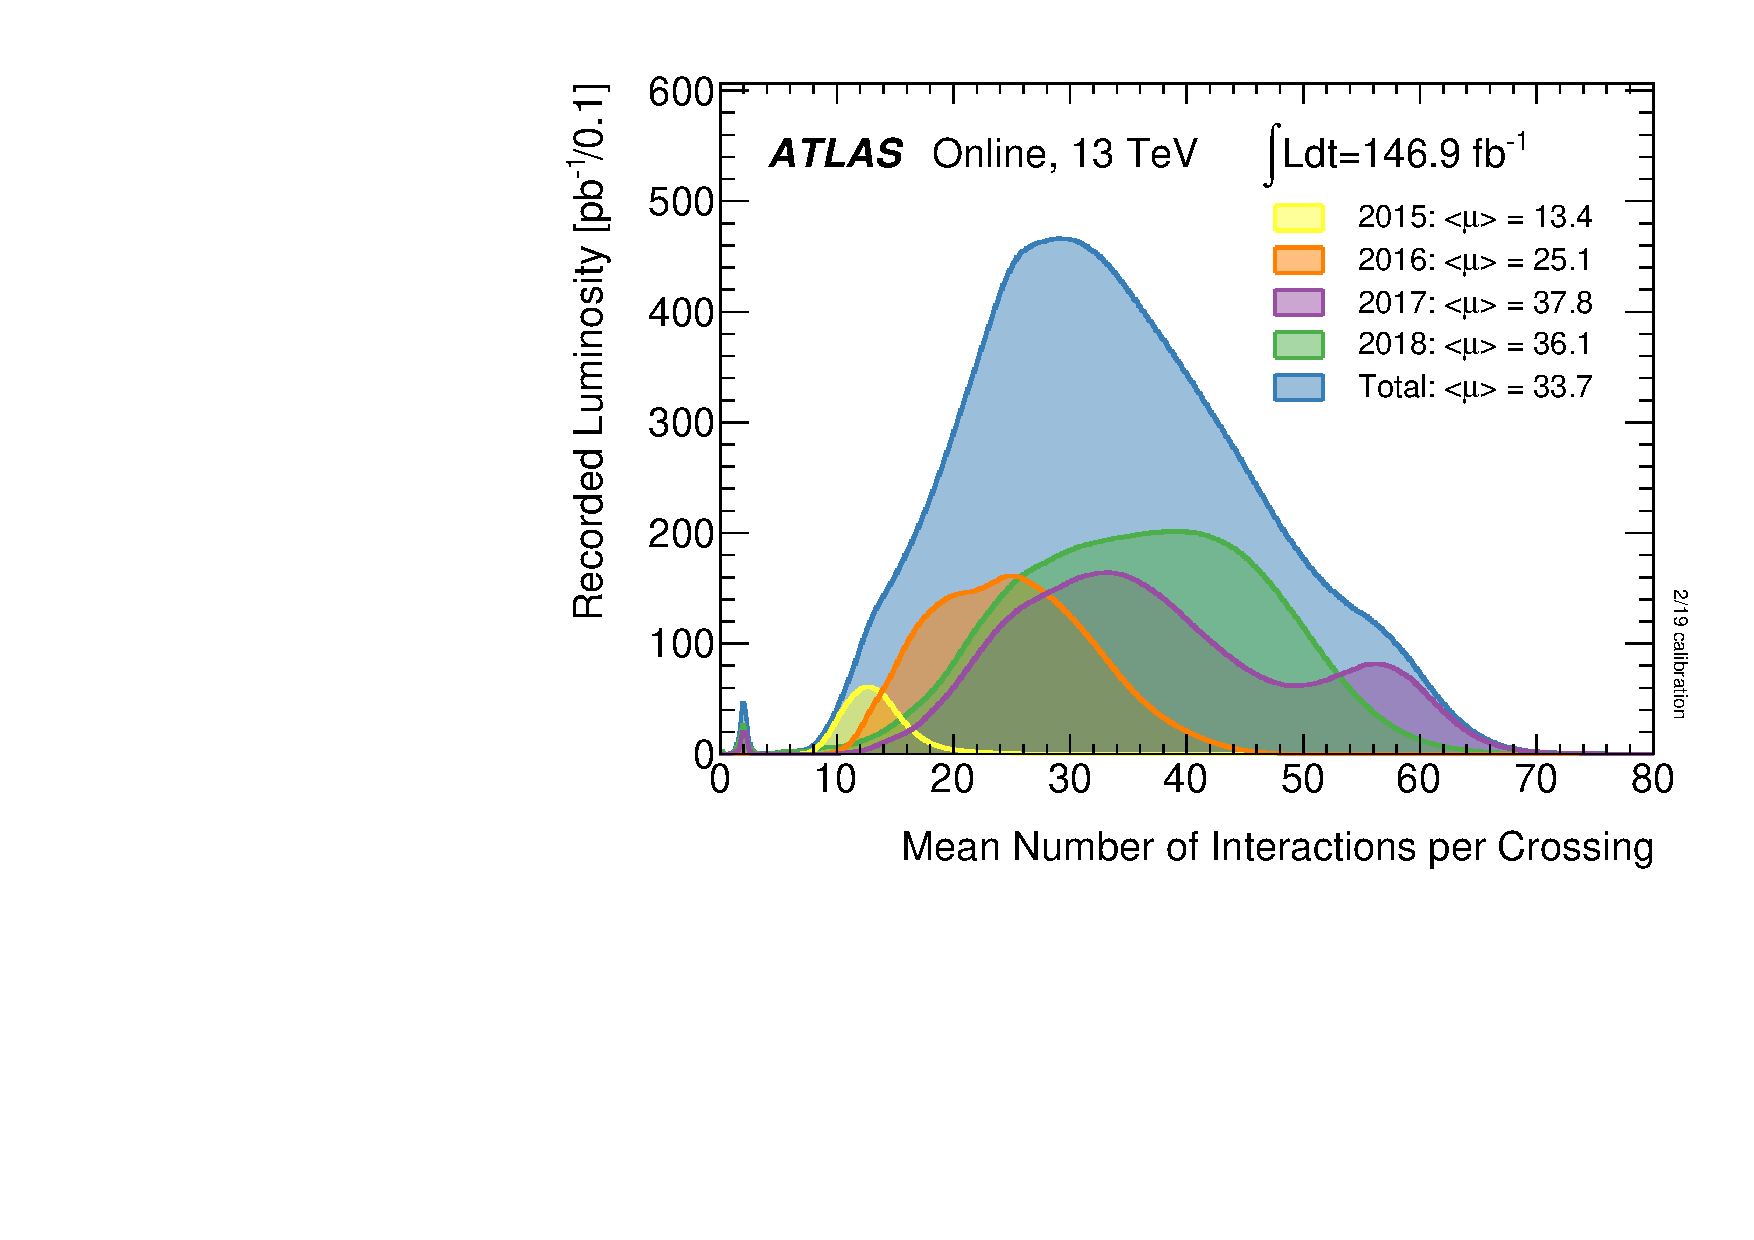
\includegraphics[width=0.7\textwidth]{mu_2015_2018}
\end{center}
\caption{
Shown is the luminosity-weighted distribution of the mean number of interactions per crossing for the 2015-2018 pp collision data at 13 TeV centre-of-mass energy.
All data recorded by ATLAS during stable beams is shown, and the integrated luminosity and the mean mu value are given in the figure.
The mean number of interactions per crossing corresponds to the mean of the poisson distribution of the number of interactions per crossing calculated for each bunch.
It is calculated from the instantaneous per bunch luminosity as $\mu = L_{\mathrm{bunch}} × \sigma_{\mathrm{inel}} / f_r$ where $L_{\mathrm{bunch}}$ is the mean per bunch instantaneous luminosity, $\sigma_{\mathrm{inel}}$ is the inelastic cross section which we take to be 80 mb for 13 TeV collisions, and $f_r$ is the LHC revolution frequency.
The luminosity shown represents the initial 13 TeV luminosity estimate and includes all 13 TeV pp data recorded up to 2018.
}
\label{fig:mu_per_year}
\end{figure}

\dots

\subsection{Signal}
\dots

\subsection{Backgrounds}
\dots

\subsubsection{QCD}
\dots

\subsubsection{$V$+jets}
\dots

\subsubsection{t$\bar{t}$}
\dots

\section{Object Selection}
\label{sec:objects}
\subsection{Large Radius Jets}
\label{sec:tccjets}
In order to identify and reconstruct potential vector boson and Higgs boson candidates, large radius parameter ("large-$R$") jets are used.
Previously the default jet algorithm in this circumstance was the \akt algorithm with a radius parameter of $R=1.0$ utilizing locally weighted topological cell clusters (LCTopo)~\cite{PERF-2014-07} for constituents.
A new jet type of jet constituent known as as Track-CaloCluster (TCC) has been developed \cite{ATL-PHYS-PUB-2017-015} which combines calorimeter and tracking data in such a way to leverage the most performant aspects of both.
In practice TCC jets exploit the superior spatial resolution of the tracker and the energy measurement of the calorimeter, respectively.
This approach is particularly beneficial for recovering angular information from highly boosted jet constituents that would otherwise merge and be lost due to the resolution limitations when using the calorimeter alone.
A comparison of jet mass and \d2 resolution is shown in Figure ~\ref{fig:tcc_lctopo_res}.
For these reasons TCC jets are used in this analysis rather than LCTopo.

Pileup dependence is removed using trimming ~\cite{Krohn:2009th} using parameters $f_{\mathrm{cut}} = 0.05$ and $R_{\mathrm{sub}} = 0.2$.
A Monte Carlo based particle-level calibration is applied to the jets used in this analysis, which corrects on average the reconstructed mass and \pt\ of the jets to their true values.

\begin{figure}[htbp!]
\begin{center}
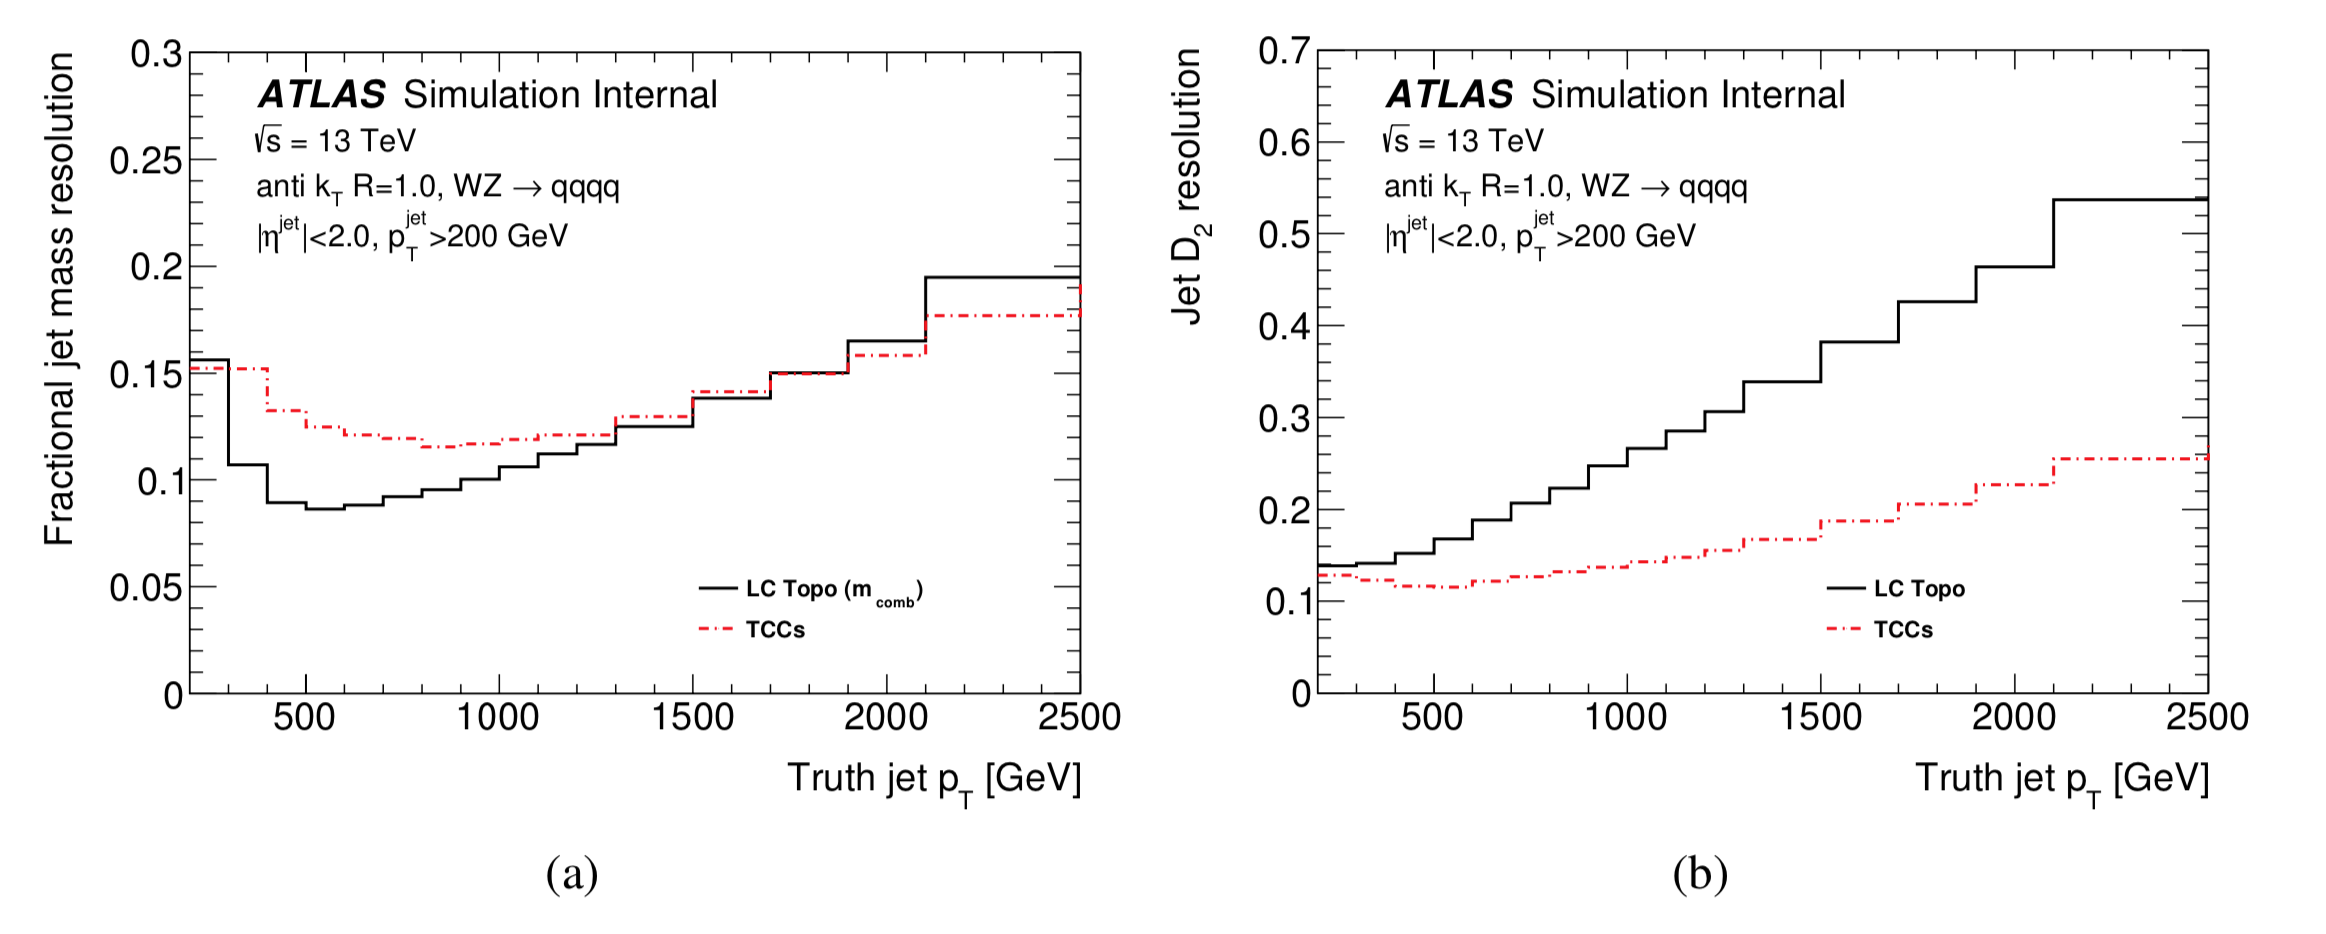
\includegraphics[width=\textwidth]{TCC_LCTopo_Mass_D2_resolution.png}
\end{center}
\caption{A comparison of the fractional jet (a) mass and (b) \d2 resolution for LCTopo (solid black lines) and TCC (dashed red lines) as a function of truth jet \pt.}
\label{fig:tcc_lctopo_res}
\end{figure}

%\TODO{reference trigger section}
All large-R jets are required to have a $p_T$ of at least 200 GeV in order to ensure the calibration is well understood.
Furthermore, each large-R jet is required to have $|\eta|<2.0$ to ensure that the track-jets associated with it are contained within the ATLAS Inner Detector volume.
The leading large-R jet must also have a $p_T$ greater than 500 GeV, ensuring that the large-R jet is in the trigger efficiency plateau for triggers used in 2015, 2016, 2017, and 2018 datasets.
The large-R jet reconstruction, calibration, and selection parameters are summarized in Table ~\ref{tab:jet_parameters}.

\begin{table}[!htb]
%\begin{scriptsize}
\begin{center}
\begin{tabular}{|c|c|c|c|}
\hline
Parameter & Value \\
\hline
Algorithm & anti-$k_T$ \\
Radius & 1.0 \\
Constituent Type & TrackCaloClusters \\
Grooming Algorithm & Trimming $(f_{\mathrm{cut}} = 0.05, R_{\mathrm{trim}} = 0.2)$ \\
Calibration Sequence & $\eta$ + JES + JMS \\
\pt\ Cut & $> 500$ GeV (leading), $> 200$ GeV (sub-leading) \\
$\left| \eta \right|$ Cut & $< 2.0$ \\
\hline
\end{tabular}
\caption{Summary of jet reconstruction and selection parameters for this analysis.}
\label{tab:jet_parameters}
\end{center}
%\end{scriptsize}
\end{table}

\subsection{Track-jets}
\label{sec:track_jets}
Track-jets are built by clustering Inner Detector tracks using the \akt algorithm.
All tracks used are required to be associated with the primary vertex of the event, defined as the vertex with the with largest $\sum p_T^2$.
The selected tracks are required to have $p_T$ greater than 500 MeV and pass a loose set of cuts, as listed in Section TODO.
In this analysis the variable-radius track jet collection is used, where the radius parameter is a function of the jet $p_{T}$ as $R=\rho/p_{T}$.
The parameter $\rho$ is set to 30 GeV, and the minimum and maximum values for the radius are set to 0.02 and 0.4, respectively \cite{ATL-PHYS-PUB-2017-010}.

When compared to calorimeter jets, the smaller $R$ parameters in track-jets coupled with the fact that tracks have better angular resolution than calorimeter clusters, mean that the decay products of highly boosted heavy objects can still be resolved.
After clustering, track-jets are then associated to the large-R calorimeter jets via ghost-association \cite{Cacciari:2008gn}.

A $b$-tagging algorithm is used to identify track-jets which are likely to contain $B$-hadrons from the Higgs boson decay. The MV2 algorithms exploit the relatively long lifetime of $B$-hadrons with respect to lighter hadrons, as well as the kinematics of the charged particle tracks.

Optimization studies were performed in order to determine the best b-tagging algorithm and working point for this search.
The MV2c10 algorithm is used with the 77\% fixed efficiency working point, as measured from $b$ jets in \tt events, which corresponds to a background rejection of 1/5 for $c$ jets and 1/112 for light jets.

\subsection{Leptons}
\label{sec:leptons}

%Based on the lepton veto applied in the $ZH\rightarrow \nu\nu b\bar{b}$ analysis, events with at least one loose lepton are rejected.
Loose muons are required to have $p_{T}>7$~GeV and fall in the central region of the detector ($|\eta|<2.5$). They are identified with the "loose" quality working point as defined in Section TODO. Track quality requirements are applied such that $|d_{0}/\sigma(d_{0})|<3$ and $|z_{0}\sin\theta|<0.5$~mm, where $d_{0}$ and $z_{0}$ are the transverse and longitudinal track impact parameters with respect to the beam line. Loose electrons are also required to have $p_{T}>7$~GeV, with a pseudo-rapidity requirement such that $|\eta|<2.47$. As with muons, requirements on the transverse and longitudinal impact parameters of the associated tracks are made. In terms of isolation, both loose electrons and loose muons are required to be "LooseTrackOnly", where a cone with radius $r(p_{T}^{\ell})=\min(0.2,10~\text{GeV}/p_{T}^{\ell})$ (0.3 for muons) is constructed around each lepton and for which the $p_{T}$-sum of all tracks with $p_{T}>500$~MeV defines the isolation $I_\ell$. A cut on $I_\ell/p_{T}^{\ell}<I_{0}$ is imposed, and $I_{0}$ is such that a flat efficiency of 99\% as a function of $p_{T}$ and $\eta$ is obtained for lepton candidates in $Z\rightarrow \ell \ell$ events.

\section{Event Selection}

\subsection{Pre-Selection}
\label{subsec:presel}

\subsubsection{Event Cleaning}
Non-collision backgrounds originating from calorimeter noise, beam halo interactions or cosmic rays can lead to spurious calorimeter signals and the reconstruction of "bad" jets. This effect can be suppressed by applying a standard jet cleaning procedure, which has been developed for 2015 data to reject jets based on their shape and timing information \cite{jetSelection} . Events are rejected if they contain at least one small radius jet (anti-$k_T$, with $R=0.4$) classified as ``bad-loose'' by the aforementioned jet cleaning criteria.
Additional vetos are applied to reject events where Tile or LAr calorimeter errors occur, as well as single event upsets in the SCT. These cuts are applied by accessing information via special flags recorded by each subdetector on a per-event basis. Incomplete events are also flagged and rejected by inspecting similar flags.
Events are also required to have at least one primary vertex with at least two tracks.

Due to the nature of the VR track jet reconstruction it is possible for one VR track jet $(i)$ to be fully contained within another $(j)$ in terms of their angular separation.
This overlap condition can be expressed with the following inequality:
\begin{equation}
    \Delta R(i,j) < \min(R_i, R_j)
\end{equation}
Any VR track jets matching this criteria are removed from consideration.
This prevents the utilization of track jets with an ambigious association of tracks for $b$-tagging, because in these cases it is likely that the $b$-tagging calibration scale factors are not correct.
See Figure~\ref{fig:vr_contain} for an illustration of this phenomenon.

\begin{figure}[htbp!]
    \begin{center}
        \subfloat[]{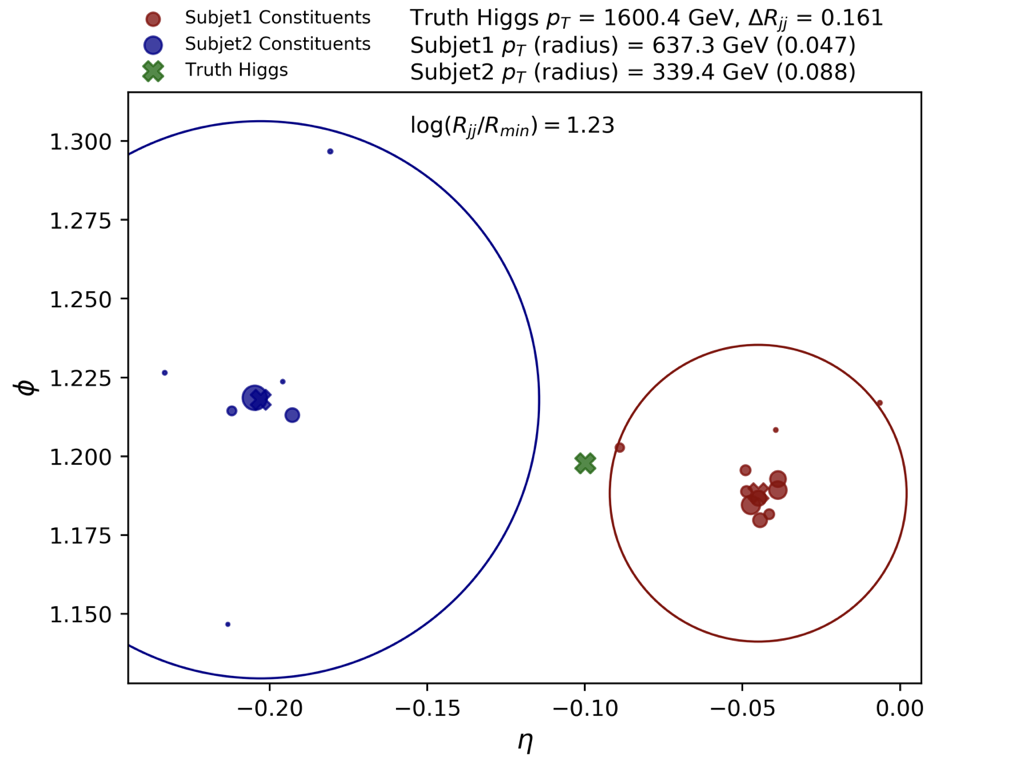
\includegraphics[width=.75\linewidth]{vr_containment_good.png}}\\
        \subfloat[]{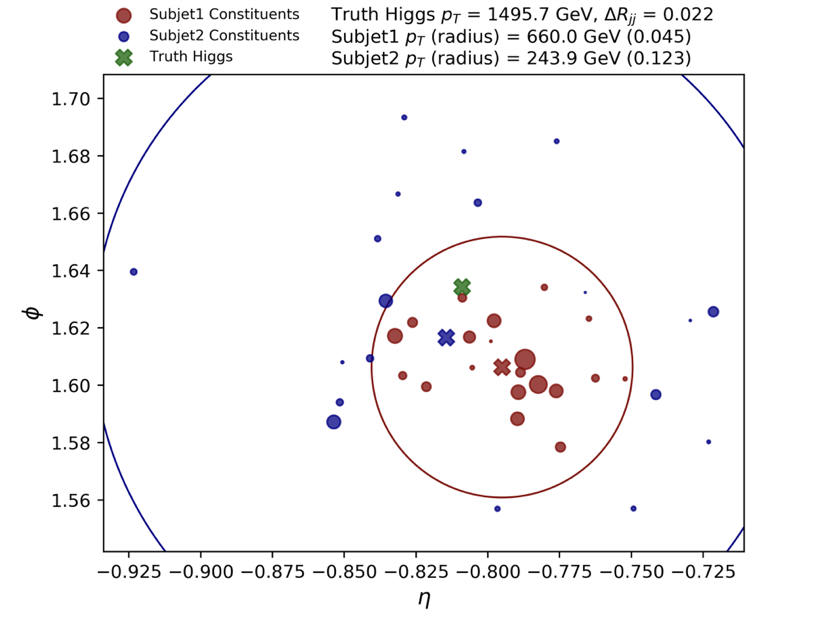
\includegraphics[width=.75\linewidth]{vr_containment_bad.png}}
    \end{center}
    \caption{ $\eta-\phi$ distribution (from simulation) of constituents of the two leading \pt VR track jets ghost associated to a truth large-R Higgs jet.
        Two illustrative cases are shown: (a) clean separation of track jet constituents and (b) pathogical overlap.
        The radii of the filled red/blue circles are proportional to $\log{\pt}$ of the corresponding track jet constituent.
    }
    \label{fig:vr_contain}
\end{figure}

\subsection{Trigger Requirements}
\label{subsec:trig}
%2015: HLT_j360_a10_lcw_sub_L1J100
%2016: HLT_j420_a10r_L1J100
%2017/2018: HLT_j460_a10t_lcw_jes_L1J100

For the analysis of the 2015 dataset, a high $p_T$, unprescaled large-$R$ jet trigger is used to trigger events: HLT\_j360\_a10\_lcw\_sub\_L1J100. During the 2016 data taking, given the increase in instantaneous luminosity, the trigger with a higher threshold is used: HLT\_j420\_a10r\_L1J100. For the 2017 and 2018 datasets an even higher threshold is used: HLT\_j460\_a10t\_lcw\_jes\_L1J100. The 2015/2016 triggers listed above fire on the untrimmed jet $p_T$, while the 2017/2018 trigger fires on the trimmed jet $p_T$ and applies a subsequent jet energy scale calibration.

For all datasets the offline selection is chosen to produce nearly 100\% efficiency. No scale factors are needed in MC to match the efficiency obtained in data.
The efficiency of the relevant triggers as a function of leading large-R jet $\pt$ are shown in Figure~\ref{fig:trigeffturnon}.

\begin{figure}[htbp!]
\begin{center}
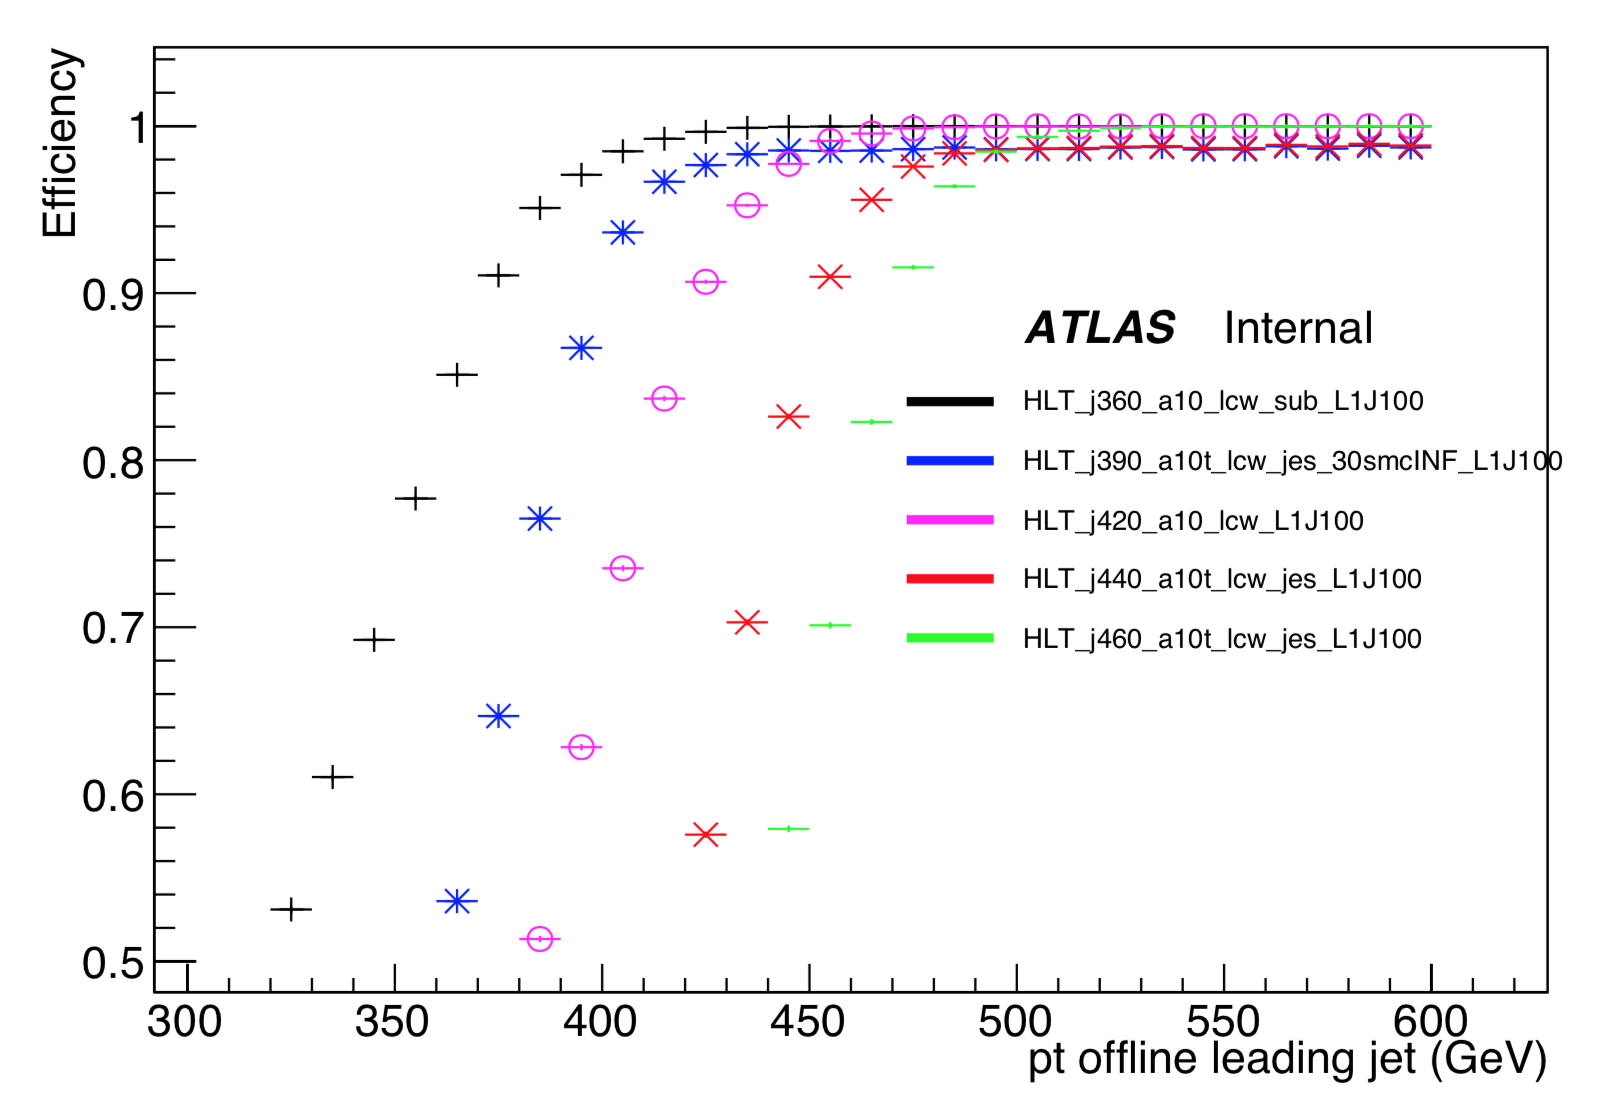
\includegraphics[width=0.49\textwidth]{trigger_eff_vs_pt.png}
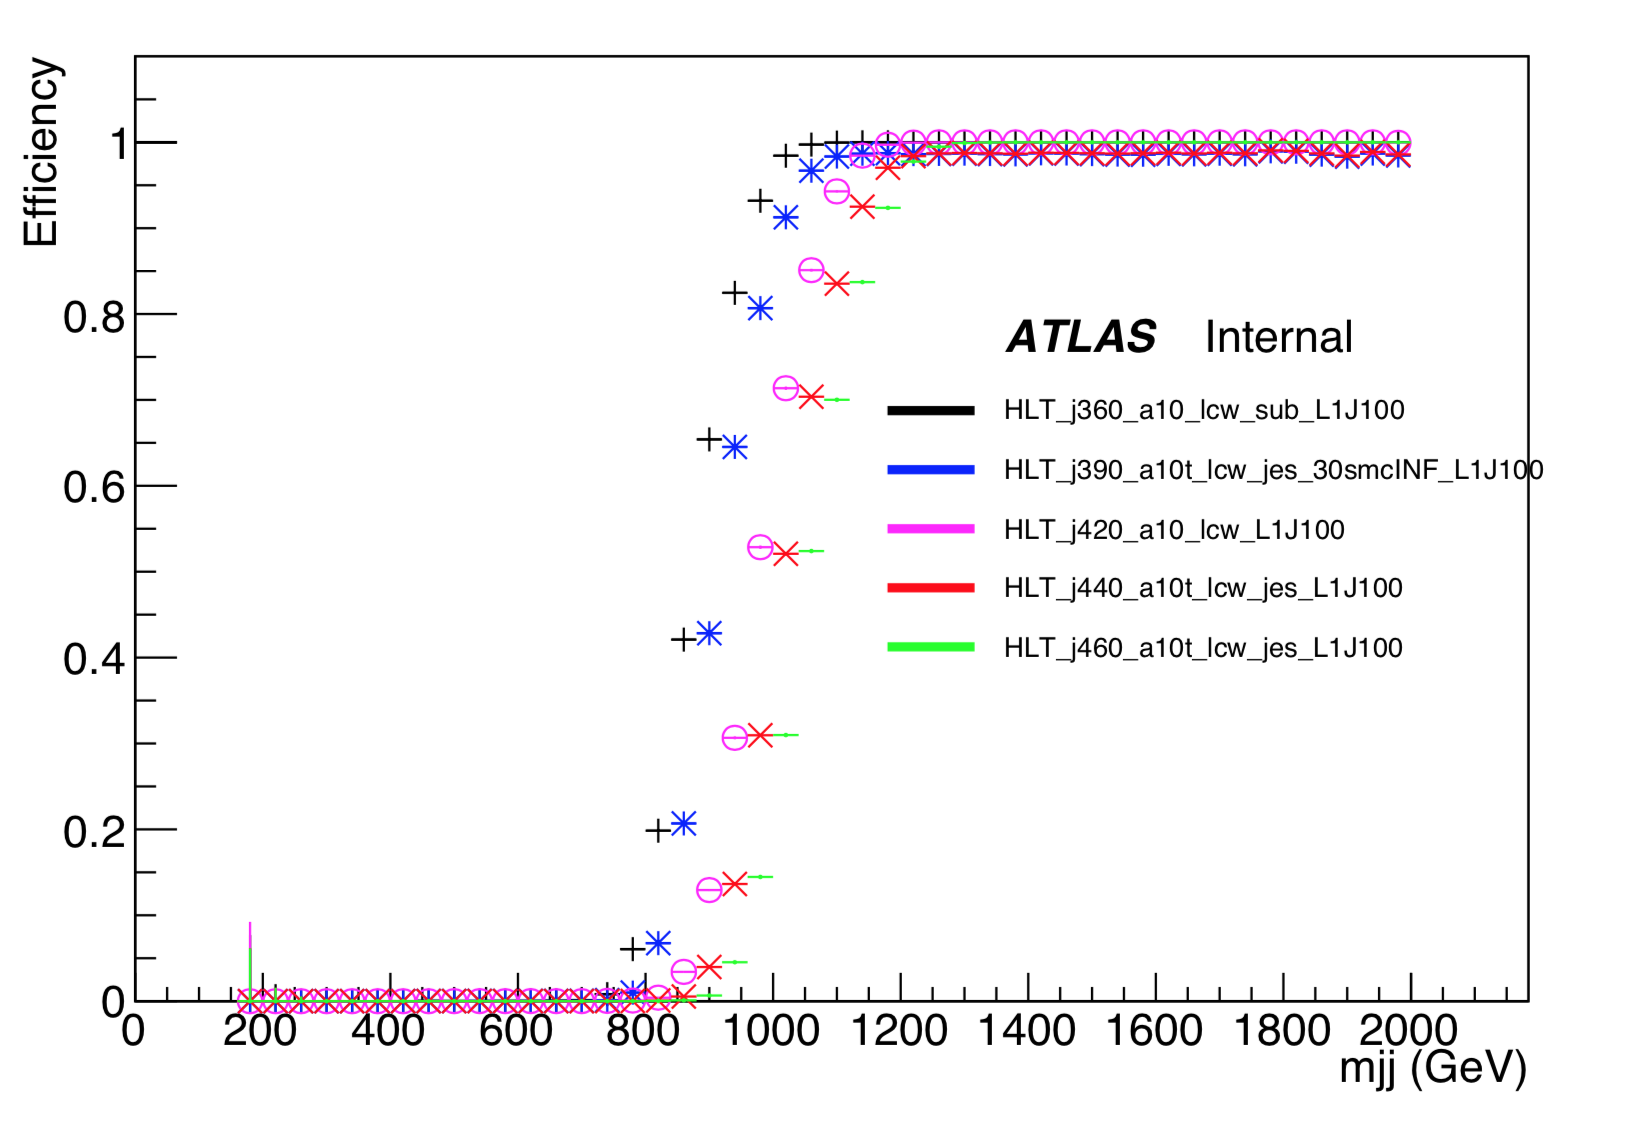
\includegraphics[width=0.49\textwidth]{trigger_eff_vs_mjj.png}
\end{center}
\caption{
    The efficiency of a range of HLT large-R jet triggers as a function of the leading large-R jet $p_T$ (left) and dijet mass (right).
    The dijet mass (right) plot is produce after applying a flat leading jet $p_T$ cut of 500 GeV.
}
\label{fig:trigeffturnon}
\end{figure}

\dots

\subsubsection{Jet Selection}
At least two large-$R$ jets are required to be present in the event which pass the kinematic cuts explained in Section \ref{sec:objects}.
In order to ensure full trigger efficiency, a cut of 500 GeV is placed on the leading large-R jet $\pt$.
The two leading jets in the event will correspond to a vector boson and a Higgs boson candidate, the assignment of which is made based on their invariant masses: the heaviest jet is chosen as the Higgs candidate and the lightest as the $W/Z$ candidate.
Previous studies of alternative methods of H/V candidate assignment have been performed and are documented in a previous support note for this analysis ~\cite{ATL-COM-PHYS-2016-482}.
The remaining $H$ or $W/Z$ specific cuts described below apply to each jet according to this assignment.
Figure \ref{fig:assignment} shows the fraction of events that are correctly matched with this V/H assignment, by checking that the jets chosen for vector and Higgs boson candidates match the truth-level bosons in the signal samples, as a function of the resonance mass.
The truth matching requirement is defined as $\Delta R < 1.0$ between the ungroomed parent of the reconstructed large radius jet and the truth hadron.

\begin{figure}[htbp!]
\begin{center}
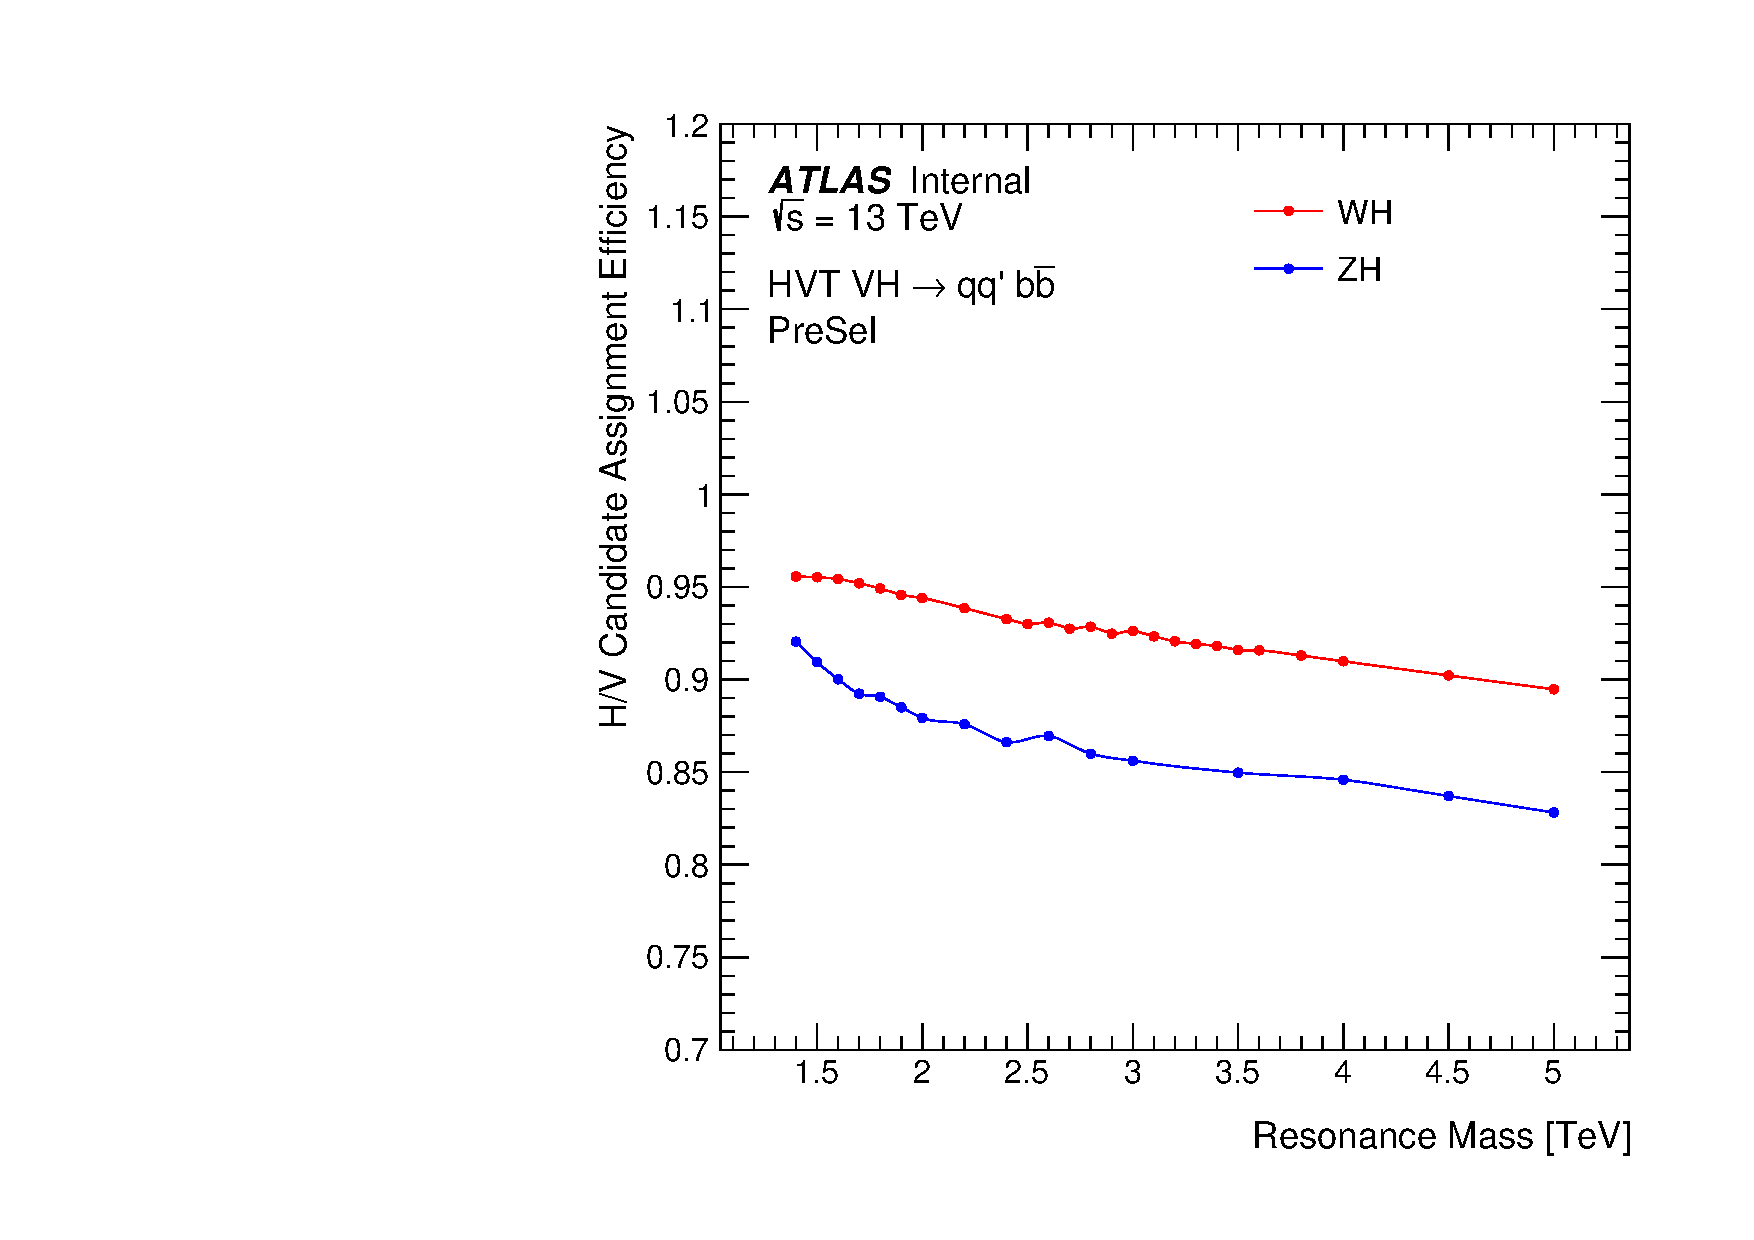
\includegraphics[width=0.49\textwidth]{VHqqbb_HVCandAssignEff_presel.pdf}
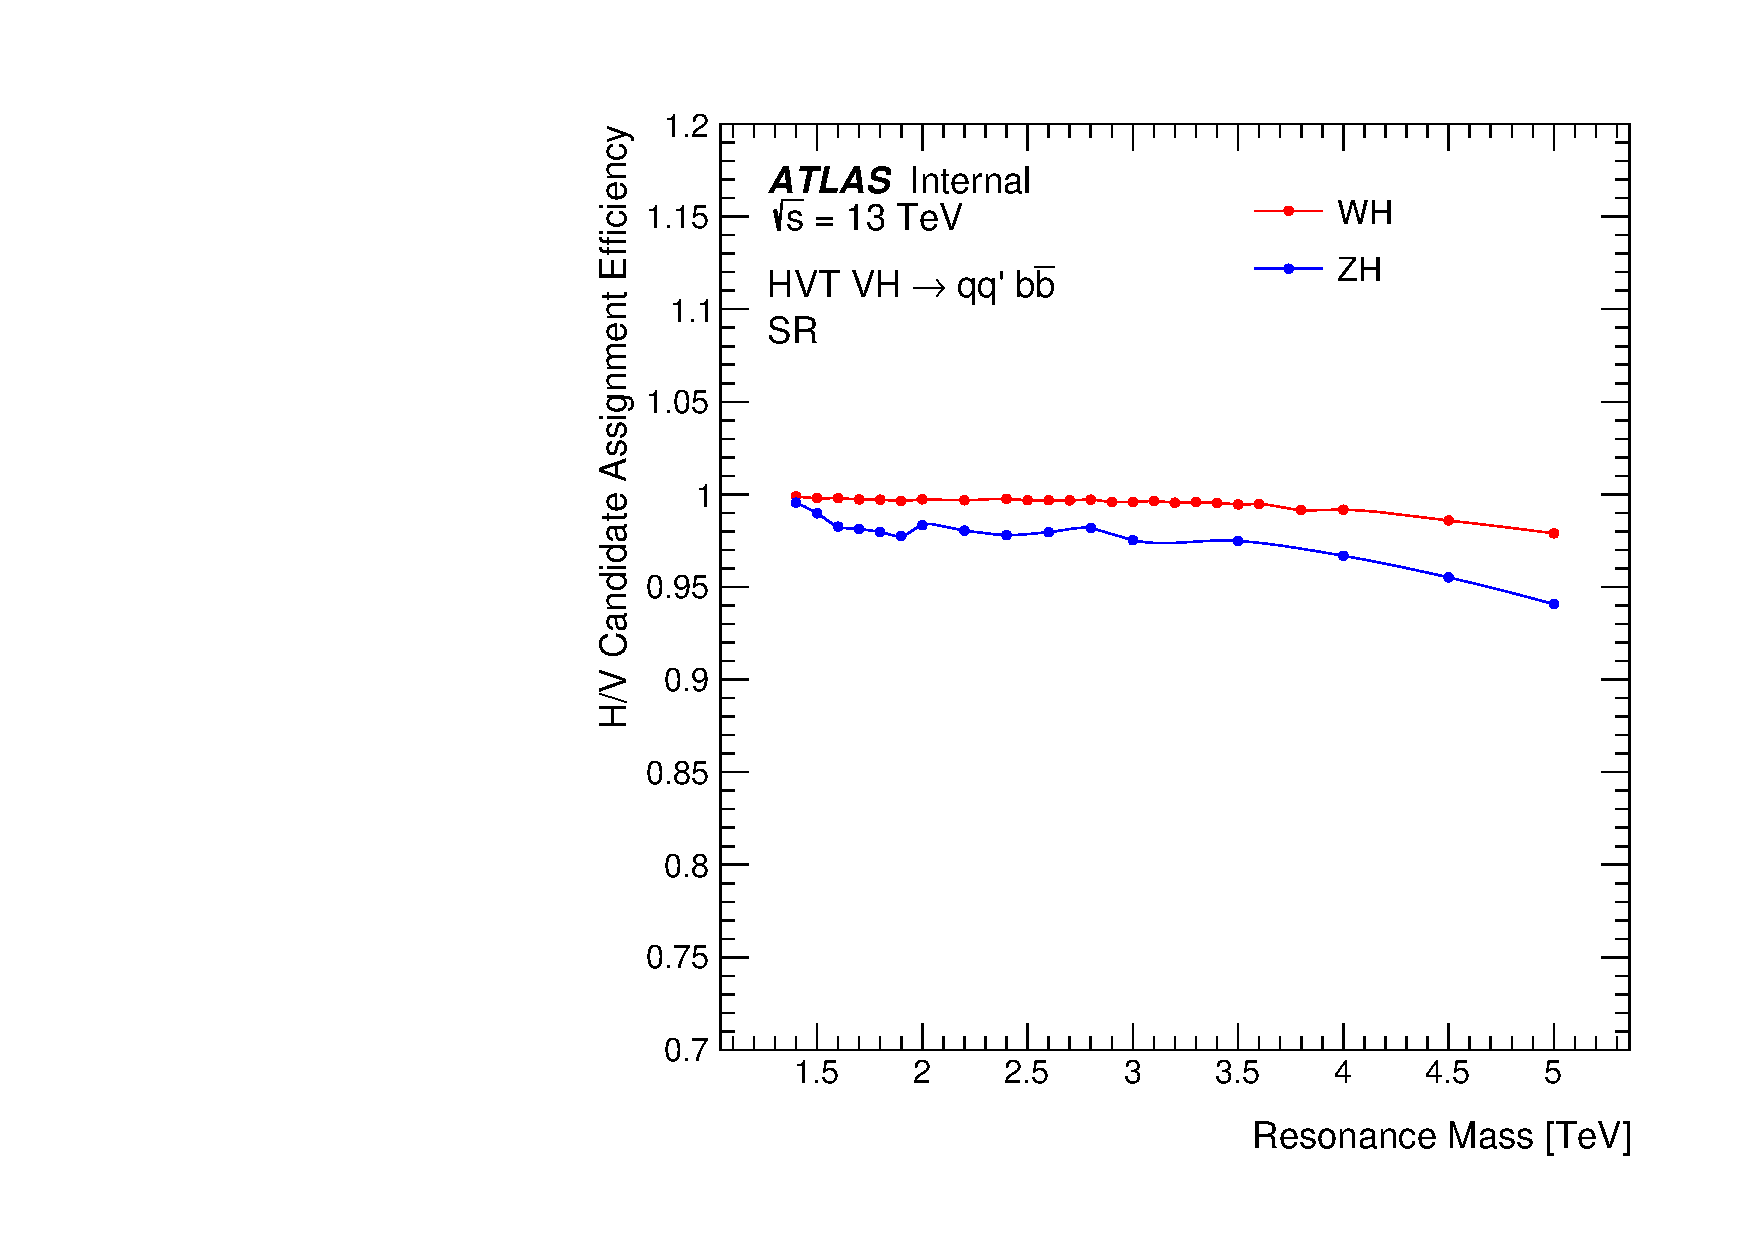
\includegraphics[width=0.49\textwidth]{VHqqbb_HVCandAssignEff_SR.pdf}
\end{center}
\caption{
Fraction of correct V/H assignments for TCC large-R jets based on the V/H assignment criteria described in the text, for $WH$ and $ZH$ signal samples, as a function of the resonance mass.
Loose pre-selection is used on the left while the combined SRWH/SRZH selection is shown on the right.
The difference in efficiency for WH vs. ZH final states is due to the closer proximity of the Higgs and Z boson masses, which produces more overlap between the optimized mass windows (see Figures~\ref{fig:vvjj_wz_tagger_mass_d2_cuts} and~\ref{fig:higgs_tagger_cuts}).
}
\label{fig:assignment}
\end{figure}

\subsubsection{Dijet Mass}
The di-jet mass of the $VH$ system, labelled \mvh or $m_{\mathrm{VH}}$, is required to be greater than 1.3 TeV in order to ensure full trigger efficiency.
A comparison of simulated background and signal distributions for \mvh\ can be found in Figure~\ref{fig:simple_mc_mVH}.

\begin{figure}[htbp!]
\begin{center}
    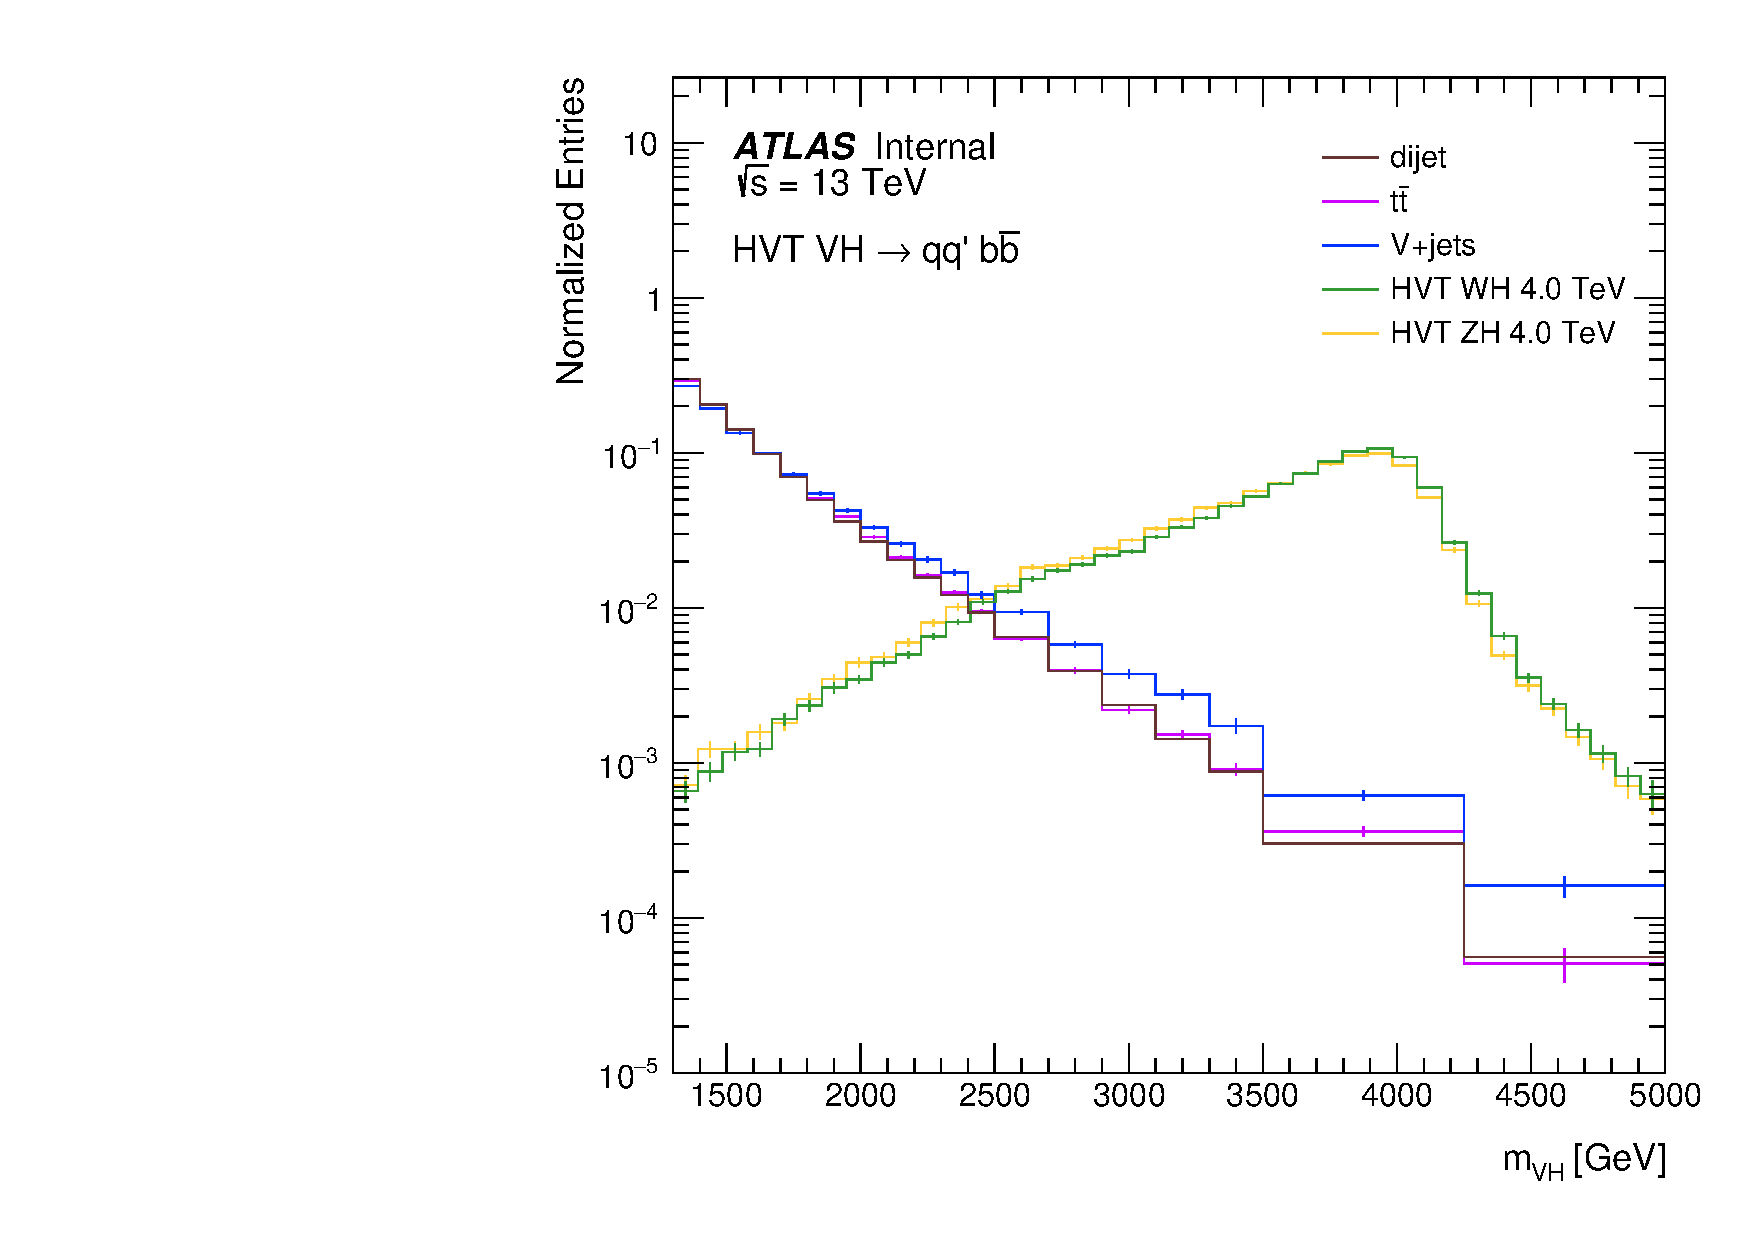
\includegraphics[width=0.49\textwidth]{VHqqbb_SimpleSigBkgMC_mVH.pdf}
\end{center}
\caption{Dijet mass \mvh, as measured in signal and background MC samples, normalized to unity.
Only pre-selection is applied, as described in Section~\ref{subsec:presel}.}
\label{fig:simple_mc_mVH}
\end{figure}

\subsubsection{Rapidity Difference}
Due to their exclusive $s$-channel production, signal \wpwh and \zpzh events are expected to be more centrally produced than QCD dijet events, resulting in a rapidity difference (\dy12) between the two leading large-$R$ jets which peaks near 0 (see Figure~\ref{fig:simple_mc_rapidity}).
Leading jets in this analysis are therefore required to have a small rapidity separation. A fixed cut of $|\Delta{y}_{12}|<1.6$ is applied.
The optimization of this cut is described in~\cite{ATL-COM-PHYS-2016-482,Summer2017}.
A comparison of simulated background and signal distributions for \dy12\ can be found in Figure~\ref{fig:simple_mc_rapidity}.

\begin{figure}[htbp!]
\begin{center}
    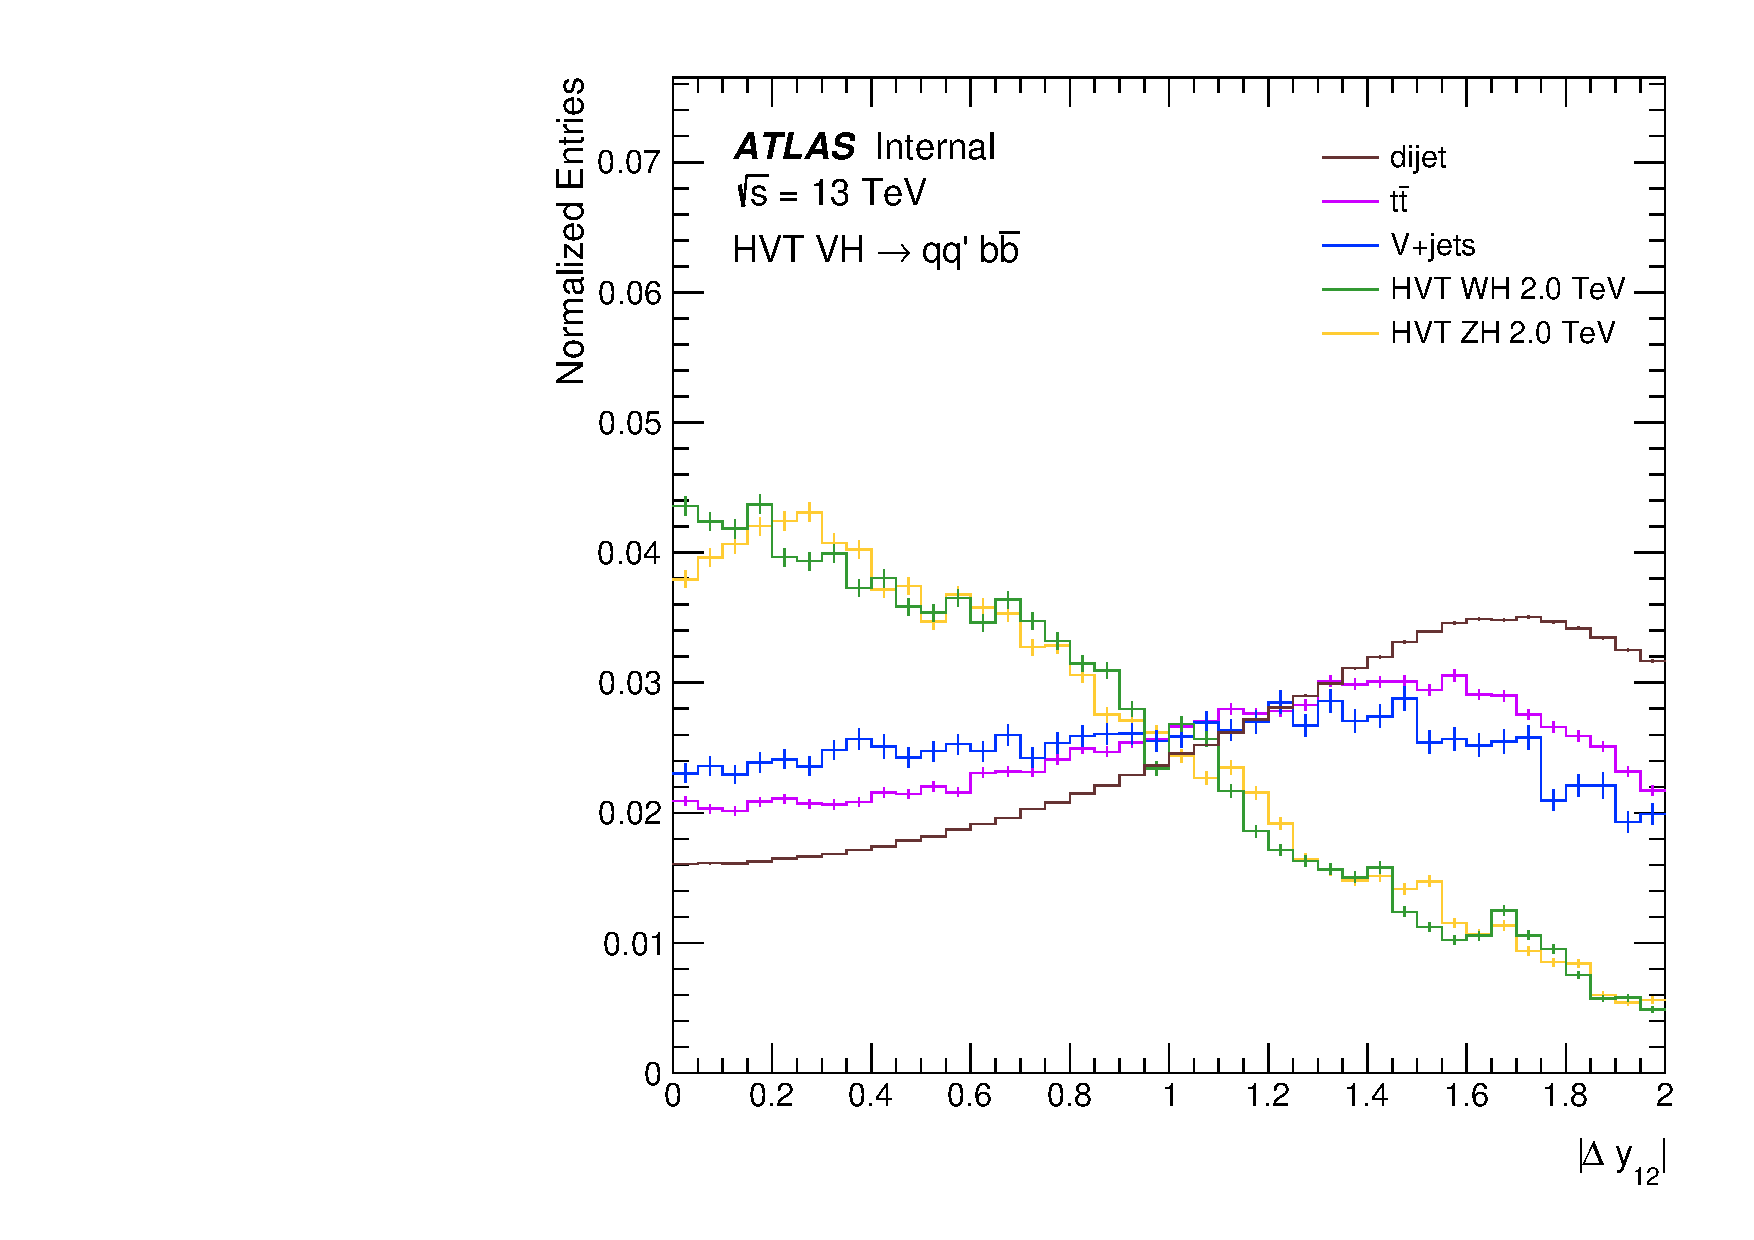
\includegraphics[width=0.49\textwidth]{VHqqbb_SimpleSigBkgMC_dyVH.pdf}
\end{center}
\caption{Rapidity difference between large-$R$ jets, as measured in signal and background MC samples, normalized to unity. Only pre-selection is applied, as described in Section~\ref{subsec:presel} }
\label{fig:simple_mc_rapidity}
\end{figure}

The cutflow and efficiencies in data for all elements of the pre-selection data can be found in Table ~\ref{tab:data_cutflow}.

\begin{table}[htbp!]
\normalsize
\centering
\begin{tabular}{c||ccc}
    Selection & Data & Efficiency [\%] & Total Efficiency [\%] \\ \hline
    EXOT3                     & 505568676 & --    & -- \\ \hline
    GRL + EventCleaning       & 483433031 & 95.62 & 95.62 \\ \hline
    Jet Cleaning              & 477623453 & 98.80 & 94.47 \\ \hline
    Trigger                   & 128220751 & 26.85 & 25.36 \\ \hline
    Jet multiplicity          & 128136392 & 99.93 & 25.35 \\ \hline
    Fatjet EtaPtPreSel        & 106779224 & 83.33 & 21.12 \\ \hline
    Lead Jet pT               & 52157511  & 48.85 & 10.32 \\ \hline
    mVH                       & 23981560  & 45.98 & 4.74 \\ \hline
    DeltaY                    & 12497837  & 52.11 & 2.47 \\ \hline
    VR Subjet Overlap Removal & 11982215  & 95.87 & 2.37 \\
\end{tabular}
\caption{
    Preselection cutflow for a subset of Run 2 data.
    The second column (Efficiency) represents the efficiency relative to the previous cut.
    The third column (Total Efficiency) represents the cumulative efficiency of all previous cuts.
}
\label{tab:data_cutflow}
\end{table}
 
\subsection{Boson Tagging}

The successful identification of \Hbb and hadronically decaying $W$/$Z$ bosons, as well as the simultaneous rejection of multijet background, relies on additional properties of the H/V candidate large-R jets. These properties are described below along with the tagging optimization method.

\subsubsection{Discriminating Variables}

\paragraph{Jet Mass}
Significant discrimination with minimal signal loss can be achieved by selecting a mass region around the resonant peak for each of the three relevant bosons.
See Figures \ref{fig:simple_mc_mV} and \ref{fig:simple_mc_mH}.

\paragraph{\d2 (W/Z tagging only)}
Jets that correspond to a hadronically decaying boson typically exhibit a two-prong structure, while QCD jets tend to exhibit a diffuse or one-prong structure.
The \d2 substructure variable used in this search to discriminate such structure is defined as a ratio of so-called \textit{energy correlation functions} \cite{Larkoski_2013} built from sums over the large-R jet constituent four-momenta.
See Figure \ref{fig:simple_mc_d2V}.
The \d2 variable provides very little additional sensitivity gain for Higgs tagging due to the redundancy with the b-tagging track jet requirements, as shown in Figure~\ref{fig:htag_sens_d2}.

\paragraph{\ntrk}
Gluon jets make up the majority of the individual large-R jets found in the QCD multijet background.
These gluon jets tend to have high hadron multiplicity due to the manner in which the QCD color factors influence the showering process.
The \ntrk variable provides a proxy measurement for charged hadron multiplicity.
It is computed from tracks passing the "loose" Inner Detector requirement with \pt > 500 MeV, $|\eta| < 2.5$, and matched to the event primary vertex.
See Figures \ref{fig:simple_mc_ntrkV} and \ref{fig:simple_mc_ntrkH}.

\paragraph{b-tagging (H only)}
The B hadrons resulting from the \Hbb decay provide an additional source of discrimination against QCD jets.
The b-tagging algorithm as described in Section \ref{sec:track_jets} is applied to the two leading \pt\ track jets ghost-associated to the Higgs candidate large-R jet.

\begin{figure}[htbp!]
\begin{center}
    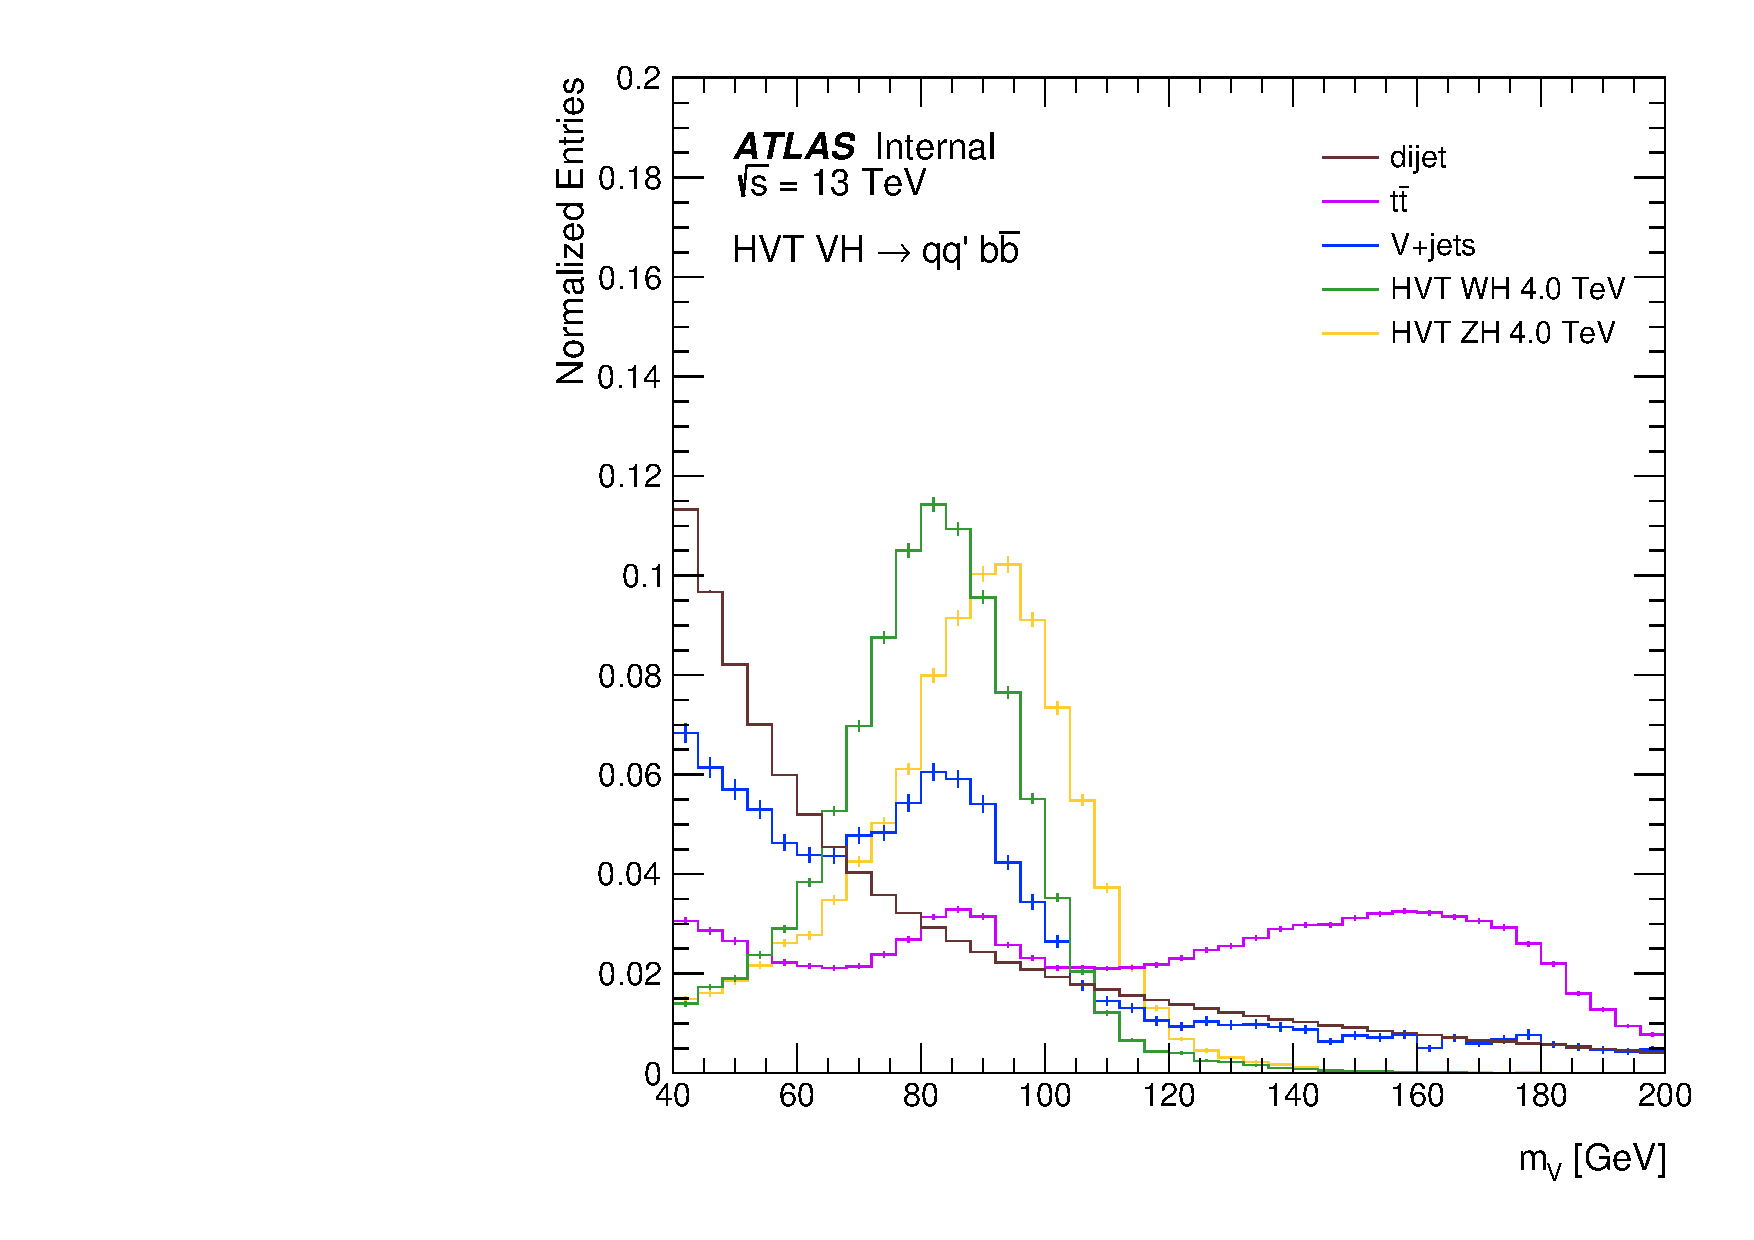
\includegraphics[width=0.49\textwidth]{VHqqbb_SimpleSigBkgMC_mV.pdf}
\end{center}
\caption{Vector boson candidate jet mass, as measured in signal and background MC samples, normalized to unity. Only pre-selection is applied, as described in Section~\ref{subsec:presel}}
\label{fig:simple_mc_mV}
\end{figure}

\begin{figure}[htbp!]
\begin{center}
    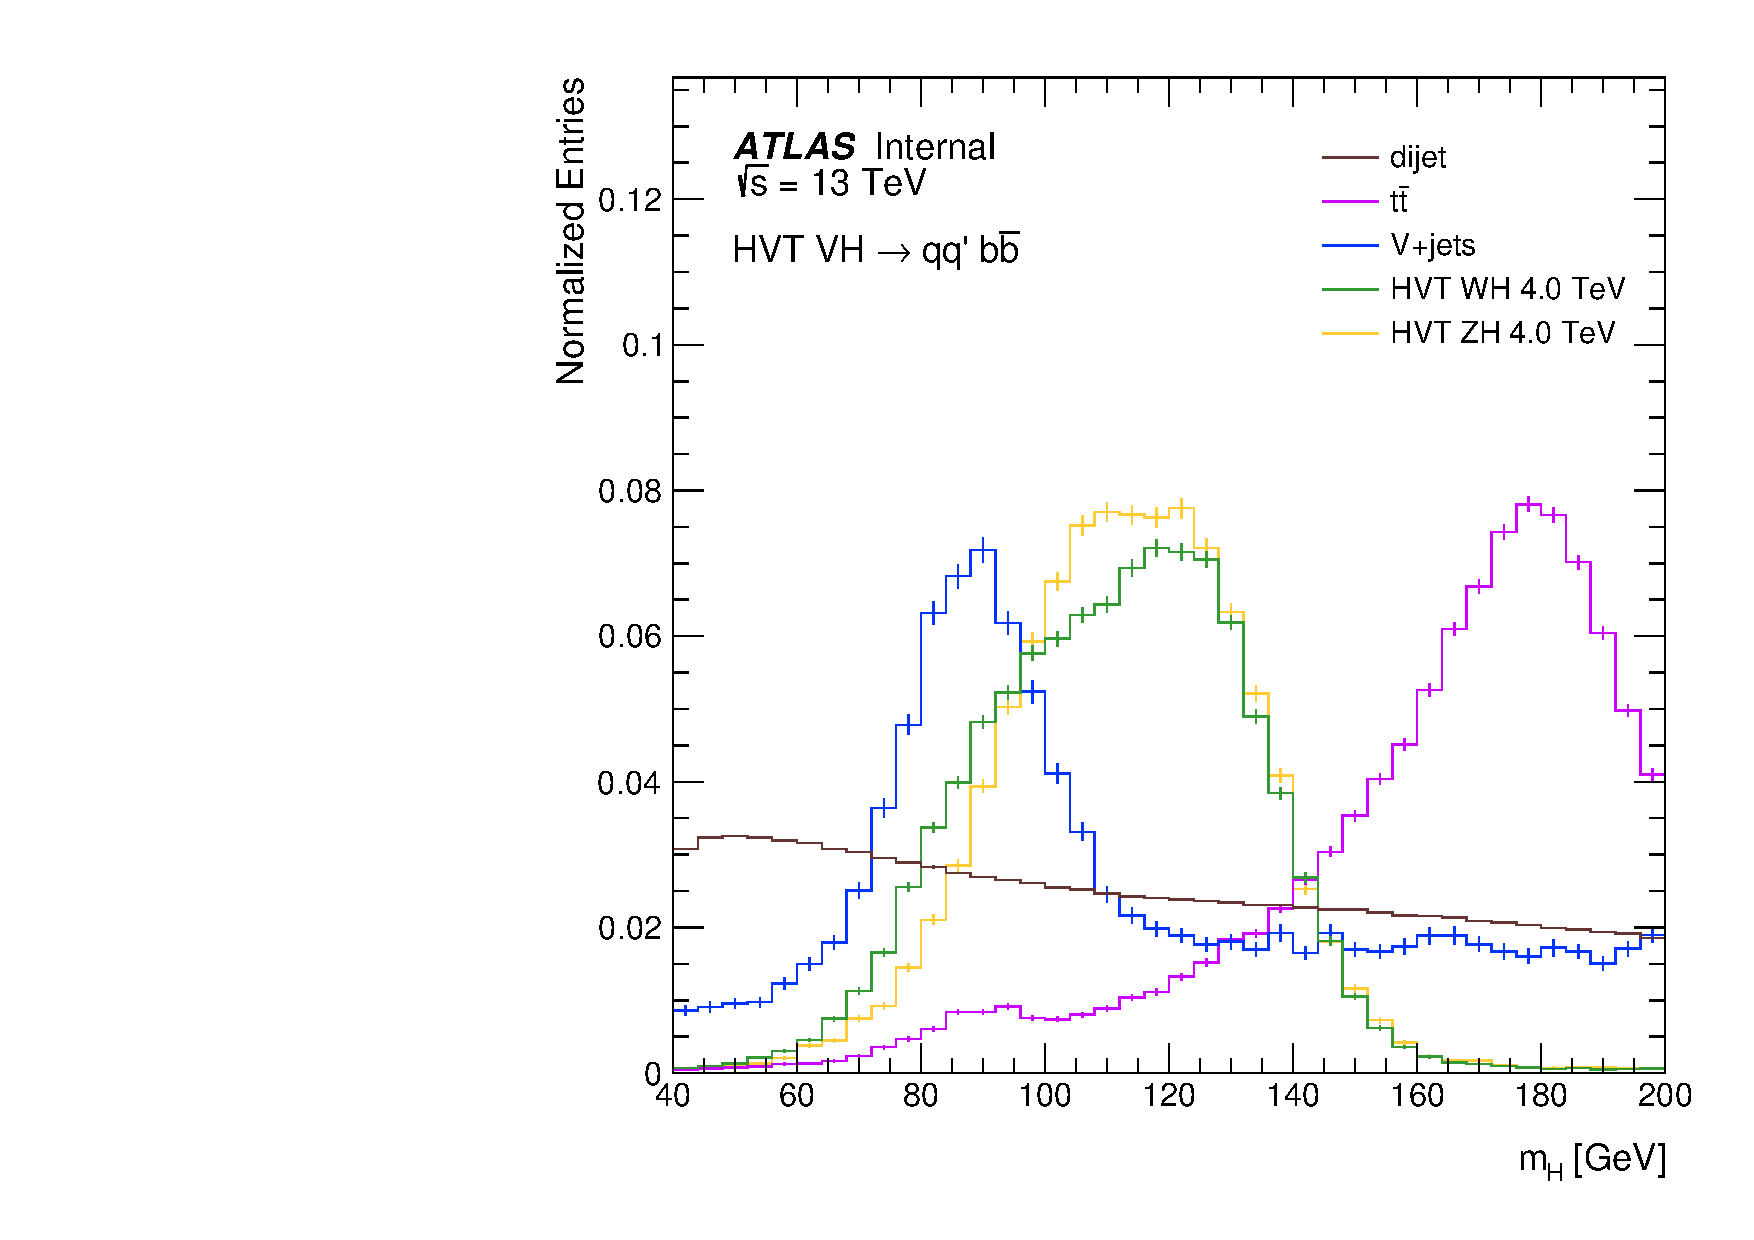
\includegraphics[width=0.49\textwidth]{VHqqbb_SimpleSigBkgMC_mH.pdf}
\end{center}
\caption{Higgs candidate jet mass, as measured in signal and background MC samples, normalized to unity. Only pre-selection is applied, as described in Section~\ref{subsec:presel} }
\label{fig:simple_mc_mH}
\end{figure}

\begin{figure}[htbp!]
\begin{center}
    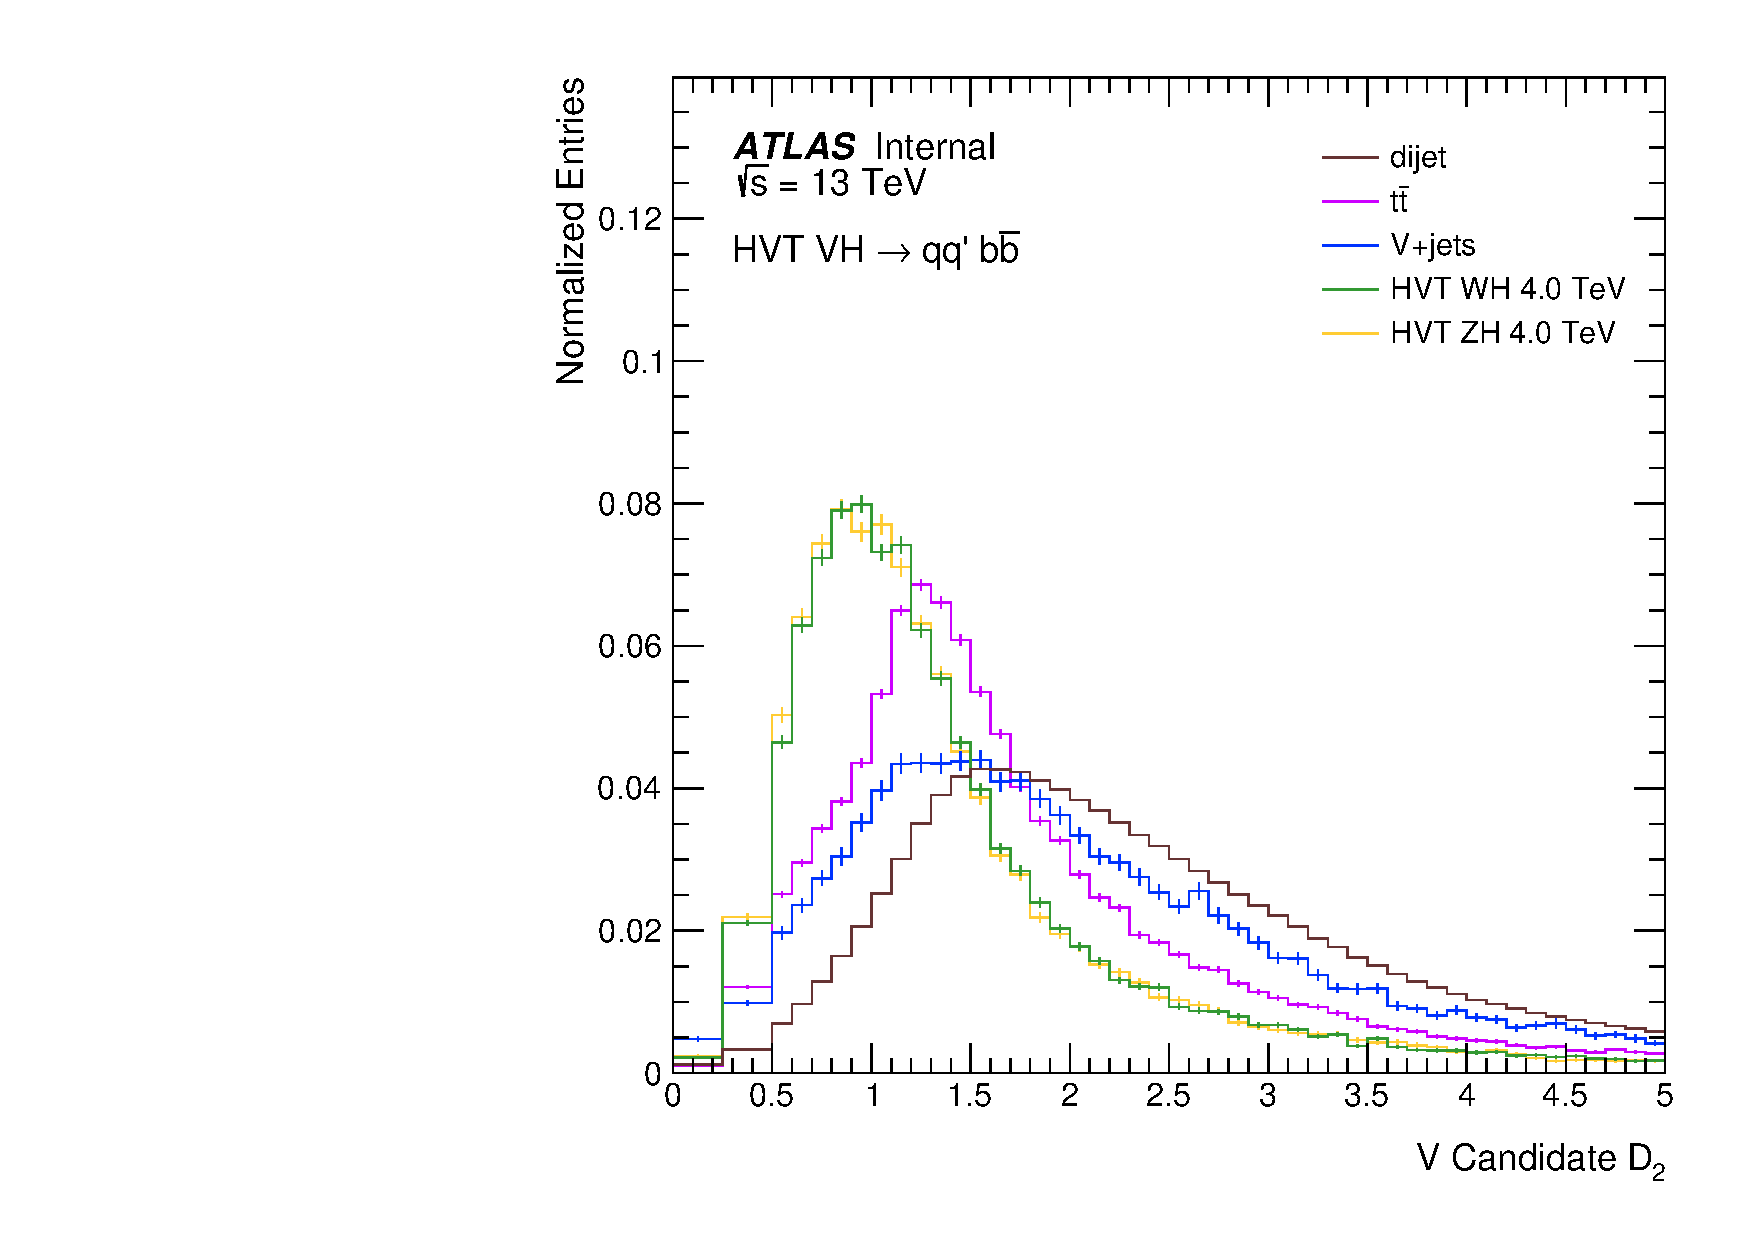
\includegraphics[width=0.49\textwidth]{VHqqbb_SimpleSigBkgMC_d2V.pdf}
\end{center}
\caption{Vector boson candidate jet \d2, as measured in signal and background MC samples, normalized to unity. Only pre-selection is applied, as described in Section~\ref{subsec:presel} }
\label{fig:simple_mc_d2V}
\end{figure}

\begin{figure}[htbp!]
\begin{center}
    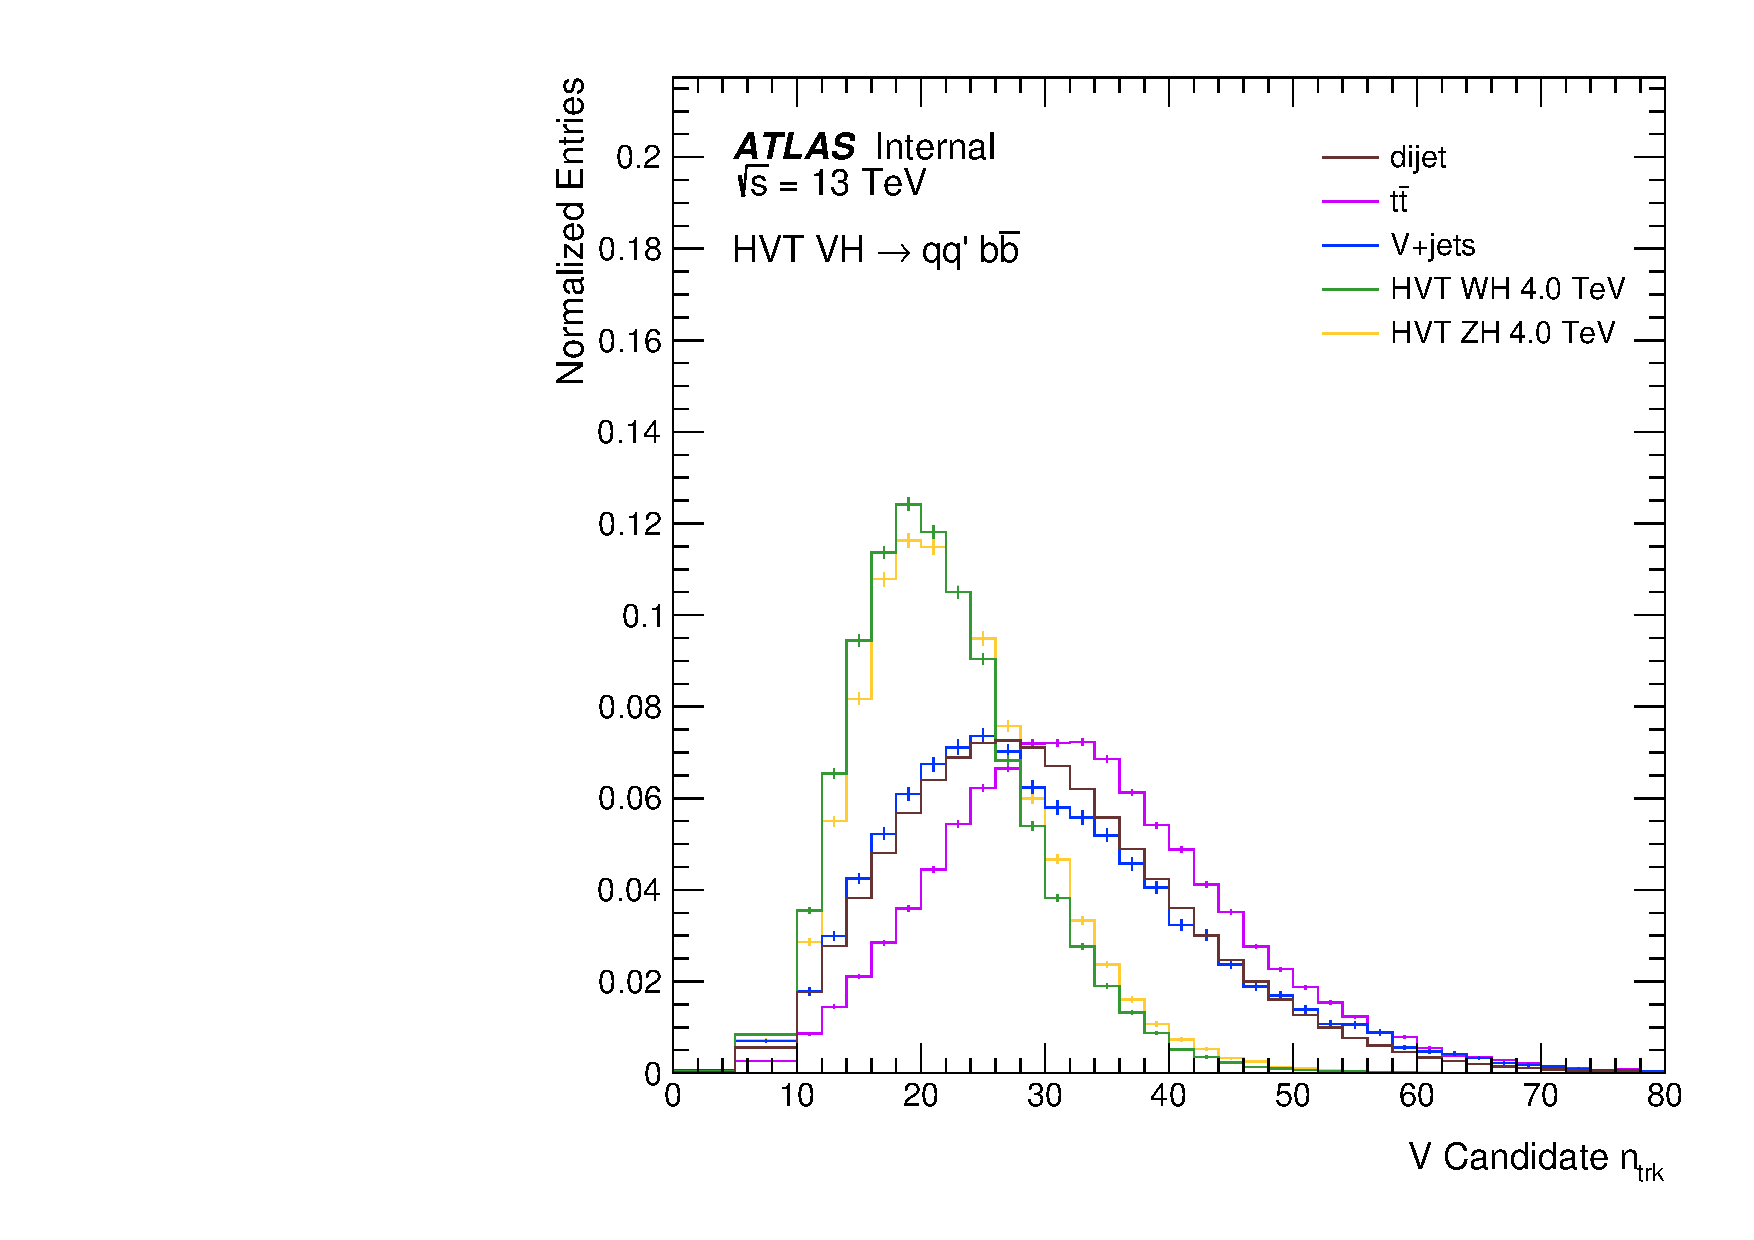
\includegraphics[width=0.49\textwidth]{VHqqbb_SimpleSigBkgMC_ntrkVVJJ_V.pdf}
\end{center}
\caption{Vector boson candidate jet \ntrk, as measured in signal and background MC samples, normalized to unity. Only pre-selection is applied, as described in Section~\ref{subsec:presel} }
\label{fig:simple_mc_ntrkV}
\end{figure}

\begin{figure}[htbp!]
\begin{center}
    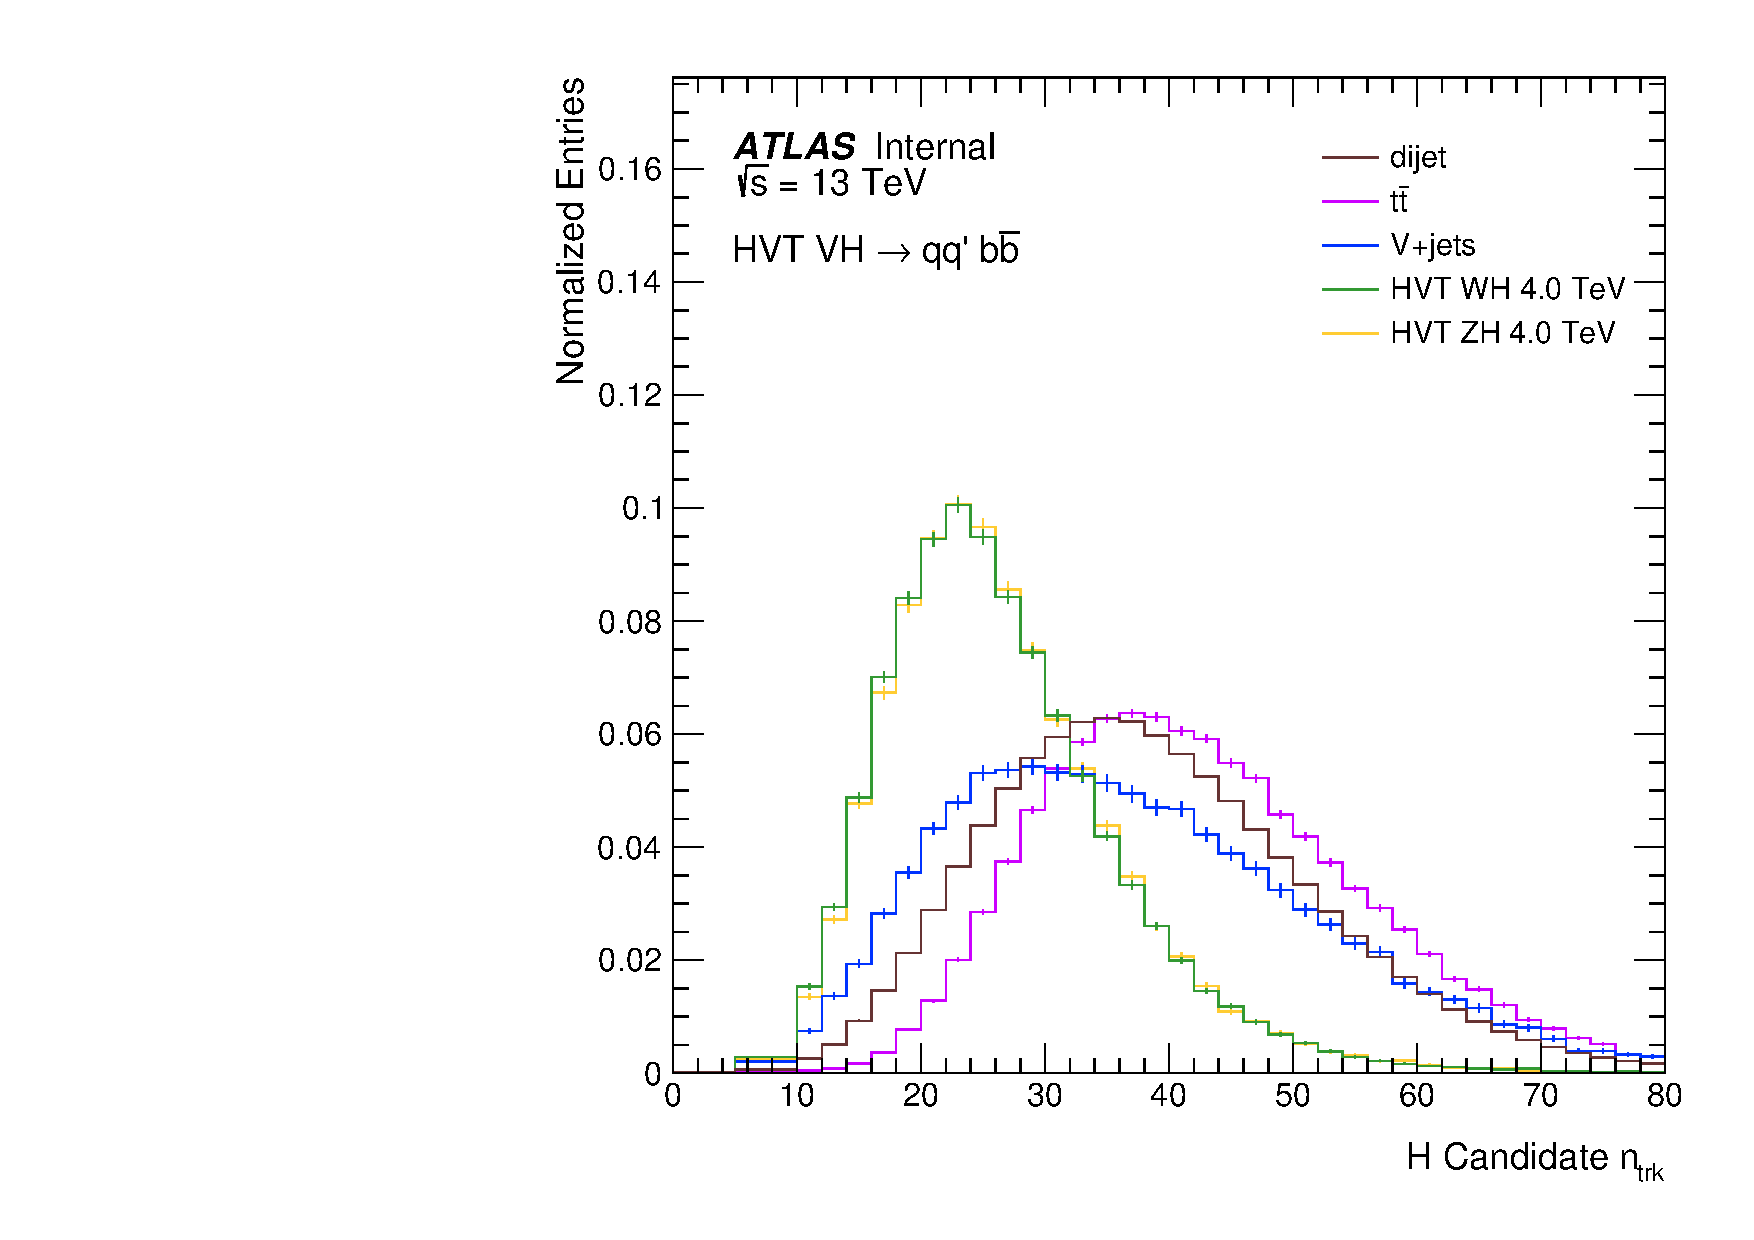
\includegraphics[width=0.49\textwidth]{VHqqbb_SimpleSigBkgMC_ntrkVVJJ_H.pdf}
\end{center}
\caption{Higgs candidate jet \ntrk, as measured in signal and background MC samples, normalized to unity. Only pre-selection is applied, as described in Section~\ref{subsec:presel} }
\label{fig:simple_mc_ntrkH}
\end{figure}

\begin{figure}[htbp!]
\begin{center}
    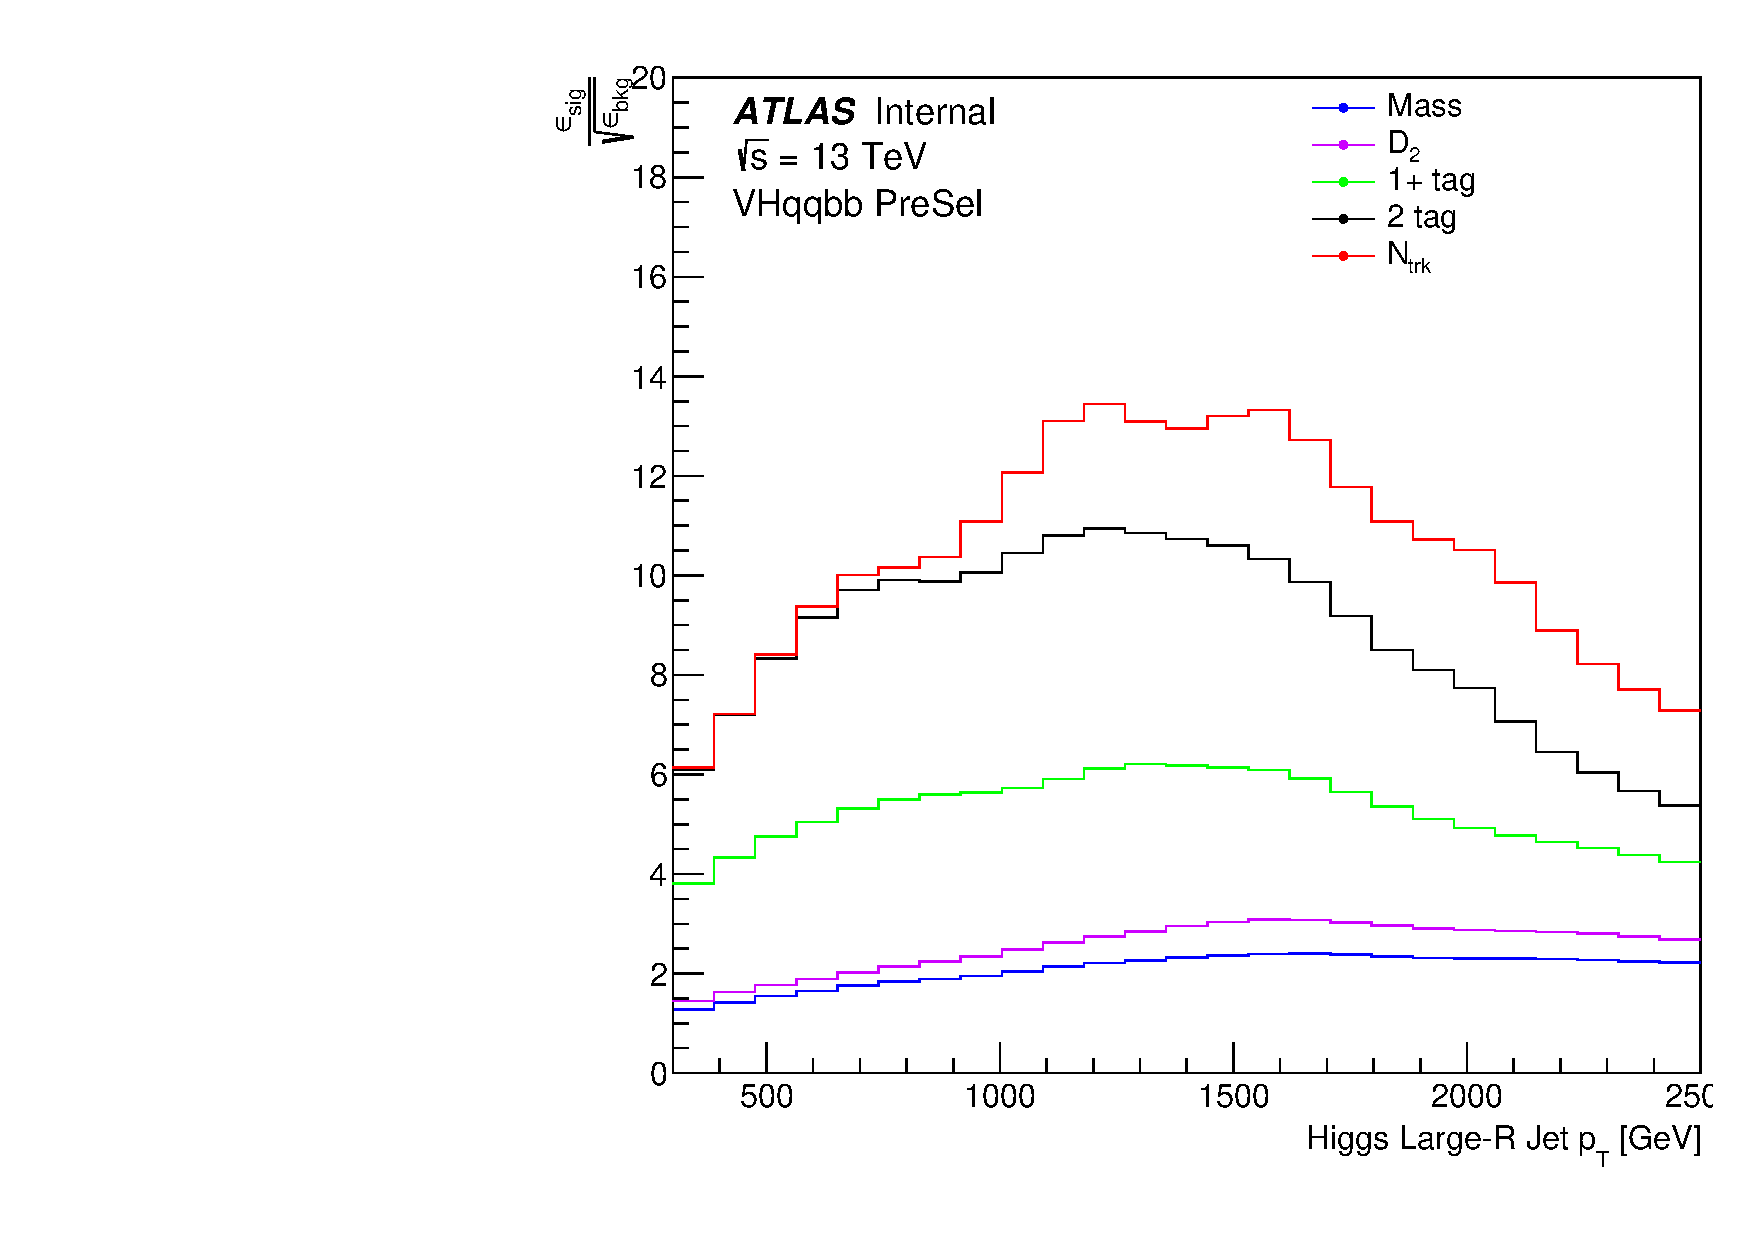
\includegraphics[width=0.49\textwidth]{PlotHTagSensitivityWithD2.pdf}
\end{center}
\caption{Sensivity of optimized cuts for Higgs tagging. The optimized \d2 cut (violet) is included only for reference and not used in the final analysis due to lack of discrimination power.
    The cuts are cumulative, in the order listed in the legend, and the pre-selection described in Section~\ref{subsec:presel} is also applied.
}
\label{fig:htag_sens_d2}
\end{figure}

\subsubsection{Optimization Method}
\label{subsec:tagger_opt}
The optimization method and motivation applied here was strongly influenced by the work done in the all-hadronic VV resonance search, and is documented in detail in the corresponding support note~\cite{VVJJSupport2019}.
For this note we only discuss the method briefly and include extra information specifically relevant to this search.

Three separate taggers are derived for W, Z, and Higgs bosons utilizing a maximum significance expression \cite{punzi2003sensitivity} which is independent of signal cross-section: $\frac{\epsilon}{\frac{a}{2}+\sqrt{B}}$, where $\epsilon$ is the signal efficiency, $a$ is the sigma count number corresponding to a one-sided Gaussian significance, and $B$ is the background yield.
Smaller values of $a$ are more appropriate for limit-setting, while larger values optimize for maximum discovery potential.
A middle ground is chosen here and a value of $a = 3$ is used.
The optimization of all variables is performed simultaneously.
The inputs to the optimization include only a loose pre-selection, without any ~\dy12 or ~\mvh cuts.
Only events with proper V/H truth matching are included in the optimization, thus $\epsilon$ represents the fraction of truth-matched W/Z/H large-$R$ ~jets passing the selection.
The words 'events' and 'jets' here are interchangeable, due to the fact that there is a maximum of one W or Z or H boson per event.
An example plot of this sensitivity expression for the $[750,950]$ GeV \pt\ bin of the Higgs tagger optimization is shown in Figure~\ref{fig:higgs_opt_sens}.

%\TODO{ cite paper this sensitivity expression is from }

For W/Z bosons a three-dimensional tagger is derived utilizing jet mass, \d2, and \ntrk.
The \d2 and \ntrk cuts are both upper bound cuts, while the jet mass cuts form a two-sided window.
In the case of Higgs tagging a two-dimensional set of jet mass and \ntrk cuts is derived.
The \d2 observable was not included in the Higgs optimization due to lack of discriminating power in conjunction with b-tagging.
For the sake of simplifying eventual combination results, the mass and \d2 cuts for the W/Z bosons derived by the VVJJ group are used.
Only the W/Z \ntrk cut is unique to this analysis, as it was shown to differ notably from VVJJ.
The primary reason for this discrepancy is that the V candidate is always the lowest mass of the two leading-\pt\ fat jets in the event, a mass-ordering that is not present for the VVJJ optimization.

Due to the correlation of each optimization variable with large-R jet \pt, each separate tagger is derived as a set of maximum sensitivity cuts in bins of large-R jet \pt.
After optimization of these cuts, they are smoothed by fitting with the following expression: $\sqrt{\frac{A^2}{(\pt-B)^2} + C^2(\pt-D)^2}$.
Both terms are first order approximations for different factors impacting the measurement resolution of the jet mass.
The first term accounts for energy resolution, which worsens at low \pt, and the second for angular resolution, which worsens at high \pt.
While this expression is physically motivated for the mass cut, it works equally well for the \ntrk cut.
Note that a separate exponential function is used by the VVJJ group to fit their \ntrk cuts ~\cite{VVJJSupport2019}.

The optimized Higgs mass and \ntrk cuts are shown in Figure ~\ref{fig:higgs_tagger_cuts}, and the successive efficiency of each cut is shown in Figure ~\ref{fig:higgs_tagger_eff}.
The optimized W/Z mass and \d2 cuts from VVJJ are shown in Figure ~\ref{fig:vvjj_wz_tagger_mass_d2_cuts}.
The optimized W/Z \ntrk cuts are shown in Figure ~\ref{fig:wz_tagger_ntrk_cuts}.


\subsection{Control/Validation Regions}
\dots

\section{BDT Re-Weighting}
\dots

\section{Background Fitting}
\dots

\section{Statistical Method}
\dots

\subsection{Overview}
% cite hypothesis testing by gregory schott from 'data analysis in high energy physics' textbook
In the absence of a discovery, The primary goal of this thesis is to place limits on a particular parameter of the HVT model: the production cross section.
This type of statistical inference is often called \textit{parameter estimation}, but more fittingly in this case, \textit{parameter constraint}. 
We begin with two hypotheses: the null hypothesis $H_0$ and the alternative hypothesis $H_1$.
In the context of a search for new physics $H_0$ is often referred to as the \textit{background-only hypothesis}, under the assumption that only Standard Model processes contribute to the observed data.
The complementary $H_1$ hypothesis, known as the \textit{signal-plus-background hypothesis}, includes the contribution of the new physics signal in addition to the Standard Model background.
For this analysis $H_1$ is in fact a family of hypotheses because both the resonance mass and production cross section are explored via continuous parameters of the HVT model.

The fundamental tool of frequentist hypothesis testing is the \textit{test statistic}, which is used to make quantitative statements about the data and its relationship to $H_0$ and $H_1$.
Given some measurements $X$, a test statistic $t(X)$ can be any (scalar, for our purposes) function.
There are, of course, desirable properties that constrain the types of functions that should be used as the test statistic.
The final conclusions about the hypotheses are based upon the comparison of the observed value of $t(X)$ to some pre-determine \textit{critical region}.
In our case of parameter constraint, the critical region is defined by a single cut value $t_c$.
It is assumed that $t$ tends to have smaller values under $H_0$ and larger values under $H_1$, and thus the critical region is $t > t_c$.

The next ingredient needed is the probability density function of $t$ under a given hypothesis $H$, $g(t|H)$.
% mention Wilks and Wald theorems

Two important quantities are defined via $g$,
\begin{align}
    \alpha &\equiv \int_{t_c}^{+ \infty} g(t|H_0)dt \\
    \beta &\equiv \int_{-\infty}^{t_c} g(t|H_1)dt
\end{align}
The probability that to reject the background-only hypothesis ($H_0$) even though it is true is given by $\alpha$.
The probability that to reject the signal-plus-background hypothesis ($H_1$) even though it is true is given by $\beta$.
An ideal test statistic will minimize $\beta$ for a given $\alpha$.
Often $\alpha$ is referred to as the \textit{significance level} of the test and $1-\beta$ is called the \textit{power} of the test.
For a new physics search $\alpha$ must of necessity be quite small and is typically chosen to be 5\%.
It is important to note at this point that the values of both $\alpha$ and $\beta$ are independent of the observed data $X$, rather they indicate something about the quality and characteristics of the statistical method that will eventually be applied to data.

There is some freedom allowed in the choice of $t(X)$, but when dealing in so-called \textit{simple hypotheses}, as we are here, the Neyman-Pearson lemma states that the \textit{likelihood ratio} is the most powerful test for any given significance level $\alpha$.

\subsection{CLs Method}


\section{Systematic Uncertainties}
